 %% Copyright (C) 2011, Andrea Cimino, All Rights Reserved.
 %% This file is distributed under the terms of the Creative Commons
 %% Licence Non-Commercial Share-Alike license


%% Useful stuff for separate compilation.
\ifx\ismaindoc\undefined
\providecommand{\inbpdocument}{
 \documentclass[11pt,a4paper,twoside,titlepage]{scrbook}
%%%%%%%%%%%%%%%%%%%%%%%%%%%%%%%%
%%%%%%%%%%% PACKAGES %%%%%%%%%%%
%%%%%%%%%%%%%%%%%%%%%%%%%%%%%%%%
% encoding
\usepackage[utf8x]{inputenc}
\usepackage[italian]{babel} % babel (suddivisione parole in sillabe)

\usepackage{amsfonts} % matematica
\usepackage{amsmath} % matematica
\usepackage{amssymb} % simboli vari
\usepackage{calrsfs}
\usepackage{caption}
\usepackage{enumerate}
\usepackage{extarrows} % matematica
\usepackage{keyval}
\usepackage{manfnt} % Simboli curva
\usepackage{mathtools} % matematica
\usepackage{multirow} 
\usepackage[usenames, dvipsnames]{color} % colori con nome
\usepackage[pdftex]{graphicx}
\usepackage{epstopdf} % gestione file EPS
\usepackage{wrapfig} % per figure circondate da testo
\usepackage{framed}	% teoremi framed
\usepackage{fancyhdr} % header buffi
\usepackage[T1]{fontenc} % gestione hbox e vbox
\usepackage[a4paper]{geometry}
\usepackage{microtype} % gestione hbox e vbox
\usepackage[thref, amsthm, amsmath, framed, hyperref]{ntheorem} % teoremi (avanzata)
%% \usepackage{prooftree} % gestione prof-tree
\usepackage{rotating}
\usepackage{stmaryrd}
\usepackage{subfig}
\usepackage{syntax} % syntattic stuff
\usepackage{txfonts}
\usepackage{verbatim} % migliorie al verbatim
%\usepackage{hyperref}
%% \usepackage{qtree}
\usepackage{fancyvrb}
\usepackage{listings}
\usepackage{cancel}
\usepackage{tikz}

\usepackage{bbding} %% Icons

%%%%%%%%%%%%%%%%%%%%%%%%%%%%%%%%
%%%%%%%%%%% GEOMETRY %%%%%%%%%%%
%%%%%%%%%%%%%%%%%%%%%%%%%%%%%%%%
\geometry{verbose,tmargin=2cm,bmargin=2.5cm,lmargin=2.5cm,rmargin=2cm}
\parindent0ex %% Remove paragraph indenting

%%%%%%%%%%%%%%%%%%%%%%%%%%%%%%%%
%%%%%%%%%%% CODE ENV %%%%%%%%%%%
%%%%%%%%%%%%%%%%%%%%%%%%%%%%%%%%
% codice
\newcounter{count}
\setcounter{count}{0}
\newenvironment{code}[1]
{
\color{lightgray}\hrulefill\color{code}
\stepcounter{count} {\bf\small Listato di codice \arabic{count}: {#1} }
\verbatim
}
{
\endverbatim
\color{lightgray}\hrulefill
\color{black}
\\
}

% codice semplice
\newenvironment{simplecode}
{
\color{code} \tt
}
{
\rm
}

 % Notation issues

%% Proof trees.
%\input prooftree
\newcommand*{\nohyp}{\phantom{x}}

%% C++.
\newcommand*{\Cplusplus}{{C\nolinebreak[4]\hspace{-.05em}\raisebox{.4ex}
{\tiny\bf ++}}}

%% BNF rules.
\newcommand*{\vbar}{\mathrel{\mid}}

%% Abstract syntax of the analyzed language.
\newcommand*{\Type}{\mathrm{Type}}
\newcommand*{\dType}{\mathrm{dType}}
\newcommand*{\dT}{\mathrm{dT}}
\newcommand*{\sType}{\mathrm{sType}}
\newcommand*{\sT}{\mathrm{sT}}
\newcommand*{\cType}{\mathrm{cType}}
\newcommand*{\cT}{\mathrm{cT}}
\newcommand*{\Integer}{\mathrm{Integer}}
\newcommand*{\Bool}{\mathrm{Bool}}
\newcommand*{\Id}{\mathrm{Id}}
\newcommand*{\id}{\mathrm{id}}
\newcommand*{\rId}{\mathrm{rId}}
\newcommand*{\idx}{\mathrm{x}}
\newcommand*{\ridx}{\underline{\mathrm{x}}}
\newcommand*{\Exp}{\mathrm{Exp}}
\newcommand*{\Exps}{\mathrm{Exps}}
\newcommand*{\Decl}{\mathrm{Decl}}
\newcommand*{\exceptDecl}{\mathrm{exceptDecl}}
\newcommand*{\Catch}{\mathrm{Catch}}
\newcommand*{\Stmt}{\mathrm{Stmt}}
\newcommand*{\Label}{\mathrm{Label}}
\newcommand*{\Con}{\mathrm{Con}}
\newcommand*{\con}{\mathrm{con}}
\newcommand*{\fps}{\mathrm{fps}}
\newcommand*{\funBody}{\mathrm{Body}}
\newcommand*{\funbody}{\mathrm{body}}
\newcommand*{\main}{\mathrm{main}}
\newcommand*{\es}{\mathrm{es}}
\newcommand*{\formParams}{\mathrm{formParams}}
\newcommand*{\emptysequence}{\boxempty}
\newcommand*{\Glob}{\mathrm{Glob}}

%% Sets of configurations
\newcommand*{\NTe}{\Gamma_\mathrm{e}}
\newcommand*{\NTb}{\Gamma_\mathrm{b}}
\newcommand*{\NTd}{\Gamma_\mathrm{d}}
\newcommand*{\NTg}{\Gamma_\mathrm{g}}
\newcommand*{\NTs}{\Gamma_\mathrm{s}}
\newcommand*{\NTk}{\Gamma_\mathrm{k}}
\newcommand*{\Te}{T_\mathrm{e}}
\newcommand*{\Tb}{T_\mathrm{b}}
\newcommand*{\Td}{T_\mathrm{d}}
\newcommand*{\Tg}{T_\mathrm{g}}
\newcommand*{\Ts}{T_\mathrm{s}}
\newcommand*{\Tk}{T_\mathrm{k}}

%% Lambda notation.
\newcommand*{\lambdaop}{\mathop{\lambda}\nolimits}

%% Sets of (no better specified) configurations.
\newcommand*{\NT}[1]{\Gamma_{#1}}
\newcommand*{\NTq}{\Gamma_q}
\newcommand*{\Tq}{T_q}

%% Denotable values.
\newcommand*{\dVal}{\mathrm{dVal}}
%% Storeable values.
\newcommand*{\sVal}{\mathrm{sVal}}
\newcommand*{\sval}{\mathrm{sval}}

%% Control modes.
\newcommand*{\CtrlMode}{\mathord{\mathrm{CtrlMode}}}
\newcommand*{\cm}{\mathrm{cm}}
%% Branch modes.
%\newcommand*{\BranchMode}{\mathord{\mathrm{BranchMode}}}
\newcommand*{\GotoMode}{\mathord{\mathrm{GotoMode}}}
\newcommand*{\SwitchMode}{\mathord{\mathrm{SwitchMode}}}
\newcommand*{\cmgoto}{\mathop{\mathrm{goto}}\nolimits}
\newcommand*{\cmswitch}{\mathop{\mathrm{switch}}\nolimits}
\newcommand*{\cmbreak}{\mathop{\mathrm{break}}\nolimits}
\newcommand*{\cmcontinue}{\mathop{\mathrm{continue}}\nolimits}
\newcommand*{\cmreturn}{\mathop{\mathrm{return}}\nolimits}
%% Exec mode.
\newcommand*{\cmexec}{\mathrm{exec}}
%% Value mode.
\newcommand*{\ValMode}{\mathord{\mathrm{ValMode}}}
\newcommand*{\cmvalue}{\mathop{\mathrm{value}}\nolimits}
%% Environment mode.
\newcommand*{\EnvMode}{\mathord{\mathrm{EnvMode}}}
\newcommand*{\cmenv}{\mathrm{env}}
%% Exception modes.
\newcommand*{\ExceptMode}{\mathord{\mathrm{ExceptMode}}}
\newcommand*{\cmexcept}{\mathrm{except}}

%% Control states.
\newcommand*{\CtrlState}{\mathord{\mathrm{CtrlState}}}
\newcommand*{\cs}{\mathord{\mathrm{cs}}}
%% Value states.
\newcommand*{\ValState}{\mathord{\mathrm{ValState}}}
\newcommand*{\valstate}{\upsilon}
%% Environment states.
%\newcommand*{\EnvState}{\mathord{\mathrm{EnvState}}}
%% Exception states.
\newcommand*{\ExceptState}{\mathord{\mathrm{ExceptState}}}
\newcommand*{\exceptstate}{\varepsilon}

%% Keywords.
\newcommand*{\kw}[1]{\mathop{\textup{\textbf{#1}}}}

\newcommand*{\bop}{\mathbin{\mathrm{bop}}}
%\newcommand*{\uop}{\mathop{\mathrm{uop}}}

%% Things that hold by definition.
\newcommand{\defrel}[1]{\mathrel{\buildrel \mathrm{def} \over {#1}}}
\newcommand{\defeq}{\defrel{=}}
\newcommand{\defiff}{\defrel{\Longleftrightarrow}}
%\newcommand{\defeq}{=}
%\newcommand{\defiff}{\Longleftrightarrow}

%% Divergence relation
\newcommand{\diverges}{\,\mathord{\buildrel \infty \over \longrightarrow}}

%% Special letters denoting sets and algebras.
\providecommand*{\Nset}{\mathbb{N}}             % Naturals
\providecommand*{\Qset}{\mathbb{Q}}             % Rationals
\providecommand*{\Zset}{\mathbb{Z}}             % Integers
\providecommand*{\Rset}{\mathbb{R}}             % Reals

%% Calligraphic alphabet.
\newcommand*{\calA}{\ensuremath{\mathcal{A}}}
\newcommand*{\calB}{\ensuremath{\mathcal{B}}}
\newcommand*{\calC}{\ensuremath{\mathcal{C}}}
\newcommand*{\calD}{\ensuremath{\mathcal{D}}}
\newcommand*{\calE}{\ensuremath{\mathcal{E}}}
\newcommand*{\calF}{\ensuremath{\mathcal{F}}}
\newcommand*{\calG}{\ensuremath{\mathcal{G}}}
\newcommand*{\calH}{\ensuremath{\mathcal{H}}}
\newcommand*{\calI}{\ensuremath{\mathcal{I}}}
\newcommand*{\calJ}{\ensuremath{\mathcal{J}}}
\newcommand*{\calK}{\ensuremath{\mathcal{K}}}
\newcommand*{\calL}{\ensuremath{\mathcal{L}}}
\newcommand*{\calM}{\ensuremath{\mathcal{M}}}
\newcommand*{\calN}{\ensuremath{\mathcal{N}}}
\newcommand*{\calO}{\ensuremath{\mathcal{O}}}
\newcommand*{\calP}{\ensuremath{\mathcal{P}}}
\newcommand*{\calQ}{\ensuremath{\mathcal{Q}}}
\newcommand*{\calR}{\ensuremath{\mathcal{R}}}
\newcommand*{\calS}{\ensuremath{\mathcal{S}}}
\newcommand*{\calT}{\ensuremath{\mathcal{T}}}
\newcommand*{\calU}{\ensuremath{\mathcal{U}}}
\newcommand*{\calV}{\ensuremath{\mathcal{V}}}
\newcommand*{\calW}{\ensuremath{\mathcal{W}}}
\newcommand*{\calX}{\ensuremath{\mathcal{X}}}
\newcommand*{\calY}{\ensuremath{\mathcal{Y}}}
\newcommand*{\calZ}{\ensuremath{\mathcal{Z}}}

%% Declarators for functions and relations.
\newcommand*{\reld}[3]{\mathord{#1}\subseteq#2\times#3}
\newcommand*{\fund}[3]{\mathord{#1}\colon#2\to#3}
\newcommand*{\pard}[3]{\mathord{#1}\colon#2\rightarrowtail#3}

%% Logical quantifiers stuff.
\newcommand{\st}{\mathrel{.}}
\newcommand{\itc}{\mathrel{:}}

%% Domain, codomain and range of a function.
\newcommand*{\dom}{\mathop{\mathrm{dom}}\nolimits}
%\newcommand*{\cod}{\mathop{\mathrm{cod}}\nolimits}
%\newcommand*{\range}{\mathop{\mathrm{range}}\nolimits}

%% Restriction of a function.
\newcommand*{\restrict}[1]{\mathop{\mid}\nolimits_{#1}}

%% Type of a constant.
\newcommand*{\type}{\mathop{\mathrm{type}}\nolimits}

%% Lubs, glbs, and fixed points.
\newcommand*{\lub}{\mathop{\mathrm{lub}}\nolimits}
%\newcommand*{\glb}{\mathop{\mathrm{glb}}\nolimits}
\newcommand*{\lfp}{\mathop{\mathrm{lfp}}\nolimits}
\newcommand*{\gfp}{\mathop{\mathrm{gfp}}\nolimits}

%% Generic widening.
\newcommand*{\widen}{\mathbin{\nabla}}

%% Set theory.
\renewcommand{\emptyset}{\varnothing}

%\newcommand*{\wpc}{\mathop{\wp_\mathrm{c}}\nolimits}
%\newcommand*{\wpf}{\mathop{\wp_\mathrm{f}}\nolimits}
%\newcommand*{\wpn}{\mathop{\wp_\mathrm{n}}\nolimits}

\newcommand*{\sseq}{\subseteq}
\newcommand*{\sseqf}{\mathrel{\subseteq_\mathrm{f}}}
\newcommand*{\sslt}{\subset}
%\newcommand*{\Sseq}{\supseteq}
%\newcommand*{\Ssgt}{\supset}

%\newcommand{\Nsseq}{\nsubseteq}

\newcommand*{\union}{\cup}
\newcommand*{\bigunion}{\bigcup}
%\newcommand*{\biginters}{\bigcap}
\newcommand*{\inters}{\cap}
\newcommand*{\setdiff}{\setminus}

\newcommand{\sset}[2]{{\renewcommand{\arraystretch}{1.2}
                      \left\{\,#1 \,\left|\,
                               \begin{array}{@{}l@{}}#2\end{array}
                      \right.   \,\right\}}}

%% Base sets.
\newcommand*{\ttv}{\mathrm{tt}}
\newcommand*{\ffv}{\mathrm{ff}}
\newcommand*{\divop}{\mathbin{/}}
\newcommand*{\modop}{\mathbin{\%}}
\newcommand*{\andop}{\mathbin{\textbf{\textup{and}}}}
\newcommand*{\orop}{\mathbin{\textbf{\textup{or}}}}
\newcommand*{\notop}{\mathop{\textbf{\textup{not}}}}

\newcommand*{\FI}{\mathop{\mathrm{FI}}\nolimits}
\newcommand*{\DI}{\mathop{\mathrm{DI}}\nolimits}
\newcommand*{\SL}{\mathop{\mathrm{SL}}\nolimits}
%\newcommand*{\match}{\mathop{\mathrm{match}}\nolimits}

\newcommand*{\Env}{\mathord{\mathrm{Env}}}
\newcommand*{\emptystring}{\mathord{\epsilon}}

%% Exceptions.
\newcommand*{\RTSExcept}{\mathord{\mathrm{RTSExcept}}}
\newcommand*{\rtsexcept}{\chi}
\newcommand*{\Except}{\mathord{\mathrm{Except}}}
\newcommand*{\except}{\xi}
\newcommand*{\none}{\mathtt{none}}
\newcommand*{\divbyzero}{\mathtt{divbyzero}}
\newcommand*{\stkovflw}{\mathtt{stkovflw}}
\newcommand*{\datovflw}{\mathtt{datovflw}}
\newcommand*{\memerror}{\mathtt{memerror}}
%\newcommand*{\inerror}{\mathtt{inerror}}
%\newcommand*{\nullptr}{\mathtt{nullptr}}
%\newcommand*{\outofboundsptr}{\mathtt{outofboundsptr}}

%% Flags for terminal configurations of catch clauses.
\newcommand*{\caught}{\mathtt{caught}}
\newcommand*{\uncaught}{\mathtt{uncaught}}

%% Static semantics.
\newcommand*{\TEnv}{\mathord{\mathrm{TEnv}}}
\newcommand*{\tinteger}{\mathrm{integer}}
\newcommand*{\tboolean}{\mathrm{boolean}}
\newcommand*{\trtsexcept}{\mathrm{rts\_exception}}

%% Memory structures.
\newcommand*{\Loc}{\mathord{\mathrm{Loc}}}
\newcommand*{\Ind}{\mathrm{Ind}}
\newcommand*{\Addr}{\mathrm{Addr}}
\newcommand*{\Map}{\mathrm{Map}}
%\newcommand*{\eMap}{\mathrm{eMap}}
\newcommand*{\Stack}{\mathord{\mathrm{Stack}}}
\newcommand*{\Mem}{\mathord{\mathrm{Mem}}}
\newcommand*{\stknew}{\mathop{\mathrm{new}_\mathrm{s}}\nolimits}
\newcommand*{\datnew}{\mathop{\mathrm{new}_\mathrm{d}}\nolimits}
\newcommand*{\txtnew}{\mathop{\mathrm{new}_\mathrm{t}}\nolimits}
\newcommand*{\heapnew}{\mathop{\mathrm{new}_\mathrm{h}}\nolimits}
\newcommand*{\heapdel}{\mathop{\mathrm{delete}_\mathrm{h}}\nolimits}
\newcommand*{\datcleanup}{\mathop{\mathrm{cleanup}_\mathrm{d}}\nolimits}
\newcommand*{\smark}{\mathop{\mathrm{mark}_\mathrm{s}}\nolimits}
\newcommand*{\sunmark}{\mathop{\mathrm{unmark}_\mathrm{s}}\nolimits}
\newcommand*{\slink}{\mathop{\mathrm{link}_\mathrm{s}}\nolimits}
\newcommand*{\sunlink}{\mathop{\mathrm{unlink}_\mathrm{s}}\nolimits}
\newcommand*{\asmark}{\mathop{\mathrm{mark}_\mathrm{s}^\sharp}\nolimits}
\newcommand*{\asunmark}{\mathop{\mathrm{unmark}_\mathrm{s}^\sharp}\nolimits}
\newcommand*{\aslink}{\mathop{\mathrm{link}_\mathrm{s}^\sharp}\nolimits}
\newcommand*{\asunlink}{\mathop{\mathrm{unlink}_\mathrm{s}^\sharp}\nolimits}
\newcommand*{\aswiden}{\mathop{\mathrm{widen}}\nolimits}
\newcommand*{\sm}{\dag}
\newcommand*{\fm}{\ddag}
\newcommand*{\topmost}{\mathop{\mathrm{tf}}\nolimits}
%% Short forms of \datcleanup, \sunmark, \sunlink for table.
\newcommand*{\datcleanupshort}{\mathop{\mathrm{cu}_\mathrm{d}}\nolimits}
\newcommand*{\sunmarkshort}{\mathop{\mathrm{um}_\mathrm{s}}\nolimits}
\newcommand*{\sunlinkshort}{\mathop{\mathrm{ul}_\mathrm{s}}\nolimits}

\newcommand*{\location}[1]{\mathord{#1 \; \mathrm{loc}}}
%\newcommand*{\saeval}{\mathop{\mathrm{aeval}}\nolimits}
%\newcommand*{\saupd}{\mathop{\mathrm{aupd}}\nolimits}
\newcommand*{\asupported}{\mathop{\mathrm{supported}^\sharp}\nolimits}
\newcommand*{\aeval}{\mathop{\mathrm{eval}^\sharp}\nolimits}
\newcommand*{\ceval}[1]{\mathop{\mathrm{eval}_{#1}}\nolimits}

%% Abstracts.
\newcommand*{\Abstract}{\mathord{\mathrm{Abstract}}}
\newcommand*{\abs}{\mathord{\mathrm{abs}}}

%% Integer part function.
\newcommand{\intp}{\mathop{\mathrm{int}}\nolimits}

%% Concrete functions and operations.
% Aritmethic
%% \newcommand*{\conadd}{\mathbin{\boxplus}}
%% \newcommand*{\consub}{\mathbin{\boxminus}}
%% \newcommand*{\conmul}{\mathbin{\boxdot}}
%% \newcommand*{\condiv}{\mathbin{\boxslash}}
%% \newcommand*{\conmod}{\mathbin{\boxbar}}
% Boolean
%% \newcommand*{\coneq}{\mathbin{\triangleq}}
%% \newcommand*{\conineq}{\mathbin{\trianglelefteq}}
%% \newcommand*{\conneg}{\mathbin{\daleth}}
%% \newcommand*{\conor}{\mathbin{\triangledown}}
%% \newcommand*{\conand}{\mathbin{\vartriangle}}
\newcommand*{\bneg}{\mathop{\neg}\nolimits}

%% Abstract functions and operations.
% Aritmethic
\newcommand*{\absuminus}{\mathop{\ominus}\nolimits}
\newcommand*{\absadd}{\mathbin{\oplus}}
\newcommand*{\abssub}{\mathbin{\ominus}}
\newcommand*{\absmul}{\mathbin{\odot}}
\newcommand*{\absdiv}{\mathbin{\oslash}}
\newcommand*{\absmod}{\mathbin{\obar}}
% Boolean
\newcommand*{\abseq}{\mathrel{\triangleq}}
\newcommand*{\absneq}{\mathrel{\not\triangleq}}
\newcommand*{\absleq}{\mathrel{\trianglelefteq}}
\newcommand*{\abslt}{\mathrel{\vartriangleleft}}
\newcommand*{\absgeq}{\mathrel{\trianglerighteq}}
\newcommand*{\absgt}{\mathrel{\vartriangleright}}
\newcommand*{\absneg}{\mathrel{\circleddash}}
\newcommand*{\absor}{\mathrel{\ovee}}
\newcommand*{\absand}{\mathrel{\owedge}}

%% Summaries for theorem-like environments
\newcommand{\summary}[1]{\textrm{\textbf{\textup{#1}}}}

%% Filter function extracting the relevant and irrelevant parts.
\newcommand*{\sel}{\mathop{\mathrm{sel}}\nolimits}
\newcommand*{\mem}{\mathop{\mathrm{mem}}\nolimits}

%% Modeling definite exceptions.
%\newcommand*{\None}{\mathrm{None}}

%% Strict Cartesian products.
\newcommand*{\stimes}{\otimes}
\newcommand*{\spair}[2]{{#1} \otimes {#2}}
%\newcommand*{\rstimes}{\rtimes}
%\newcommand*{\rspair}[2]{{#1} \rtimes {#2}}
%\newcommand*{\lstimes}{\ltimes}
%\newcommand*{\lspair}[2]{{#1} \ltimes {#2}}

%% Additional syntax for the numeric type extension supplement
\newcommand*{\iT}{\mathrm{iT}}
\newcommand*{\iType}{\mathrm{iType}}
\newcommand*{\tschar}{\mathrm{signed\_char}}
\newcommand*{\tuchar}{\mathrm{unsigned\_char}}
\newcommand*{\flcon}{\mathrm{fl}}
\newcommand*{\Float}{\mathrm{Float}}
\newcommand*{\sccon}{\mathrm{sc}}
\newcommand*{\sChar}{\mathrm{sChar}}
\newcommand*{\uccon}{\mathrm{uc}}
\newcommand*{\uChar}{\mathrm{uChar}}

%% Additional macros for the extension for extra numeric types
%% Floating point types.
\newcommand*{\tfloat}{\mathrm{float}}
%% Numeric types
\newcommand*{\nType}{\mathrm{nType}}
\newcommand*{\nT}{\mathrm{nT}}

%% Additional macros for the extension to pointer and arrays:
%% Elementary types.
\newcommand*{\eType}{\mathrm{eType}}
\newcommand*{\eT}{\mathrm{eT}}
%% Elementary values.
%\newcommand*{\eValue}{\mathrm{eVal}}
%% Array types.
\newcommand*{\aType}{\mathrm{aType}}
\newcommand*{\aT}{\mathrm{aT}}
%% Record types.
\newcommand*{\rType}{\mathrm{rType}}
\newcommand*{\rT}{\mathrm{rT}}
%% Object types.
\newcommand*{\oType}{\mathrm{oType}}
\newcommand*{\oT}{\mathrm{oT}}
%% Function types.
\newcommand*{\fType}{\mathrm{fType}}
\newcommand*{\fT}{\mathrm{fT}}
%% Memory types.
\newcommand*{\mType}{\mathrm{mType}}
\newcommand*{\mT}{\mathrm{mT}}
%% Pointer types.
\newcommand*{\pType}{\mathrm{pType}}
\newcommand*{\pT}{\mathrm{pT}}
%% Offsets.
\newcommand*{\Offset}{\mathrm{Offset}}
\newcommand*{\nooffset}{\boxempty}
\newcommand*{\indexoffset}[1]{\mathopen{\boldsymbol{[}}{#1}\mathclose{\boldsymbol{]}}}
\newcommand*{\fieldoffset}[1]{\mathop{\boldsymbol{.}}{#1}}
%% Lvalues.
\newcommand*{\lValue}{\mathrm{LValue}}
\newcommand*{\lvalue}{\mathrm{lval}}
%% Rvalues.
\newcommand*{\rValue}{\mathrm{RValue}}
\newcommand*{\rvalue}{\mathrm{rval}}
%%
\newcommand*{\pointer}[1]{{#1}\boldsymbol{\ast}}
\newcommand*{\maddress}[1]{\mathop{\&}{#1}}
\newcommand*{\indirection}[1]{\mathop{\boldsymbol{\ast}}{#1}}
%%
\newcommand*{\locnull}{\mathord{l_\mathrm{null}}}
\newcommand*{\ptrmove}{{\mathop{\mathrm{ptrmove}}\nolimits}}
\newcommand*{\ptrdiff}{{\mathop{\mathrm{ptrdiff}}\nolimits}}
\newcommand*{\ptrcmp}{{\mathop{\mathrm{ptrcmp}}\nolimits}}
%%
\newcommand*{\arraysyntax}[3]{\kw{#1} {#2} \kw{of}\,{#3}}
\newcommand*{\arraytype}[2]{\arraysyntax{array}{#1}{#2}}
\newcommand*{\firstof}{{\mathop{\mathrm{firstof}}\nolimits}}
\newcommand*{\arrayindex}{\mathop{\mathrm{index}}\nolimits}
\newcommand*{\locindex}{\mathop{\mathrm{locindex}}\nolimits}
%%
\newcommand*{\recordsyntax}[3]{\kw{#1} {#2} \kw{of}\,{#3}}
\newcommand*{\recordtype}[2]{\recordsyntax{record}{#1}{#2}}
\newcommand*{\field}{\mathop{\mathrm{field}}\nolimits}
\newcommand*{\locfield}{\mathop{\mathrm{locfield}}\nolimits}
%%
\newcommand*{\NTo}{\Gamma_\mathrm{o}}
\newcommand*{\To}{T_\mathrm{o}}
\newcommand*{\NTl}{\Gamma_\mathrm{l}}
\newcommand*{\Tl}{T_\mathrm{l}}
%\newcommand*{\NTr}{\Gamma_\mathrm{r}}
%\newcommand*{\Tr}{T_\mathrm{r}}
%%
\newcommand*{\arraydatnew}{\mathop{\mathrm{newarray}_\mathrm{d}}\nolimits}
\newcommand*{\arraystknew}{\mathop{\mathrm{newarray}_\mathrm{s}}\nolimits}
\newcommand\Cut{\using\sf cut\thickness.08em\justifies}
\newcommand{\maybeeq}{\mathrel{\buildrel \mathrm{?} \over =}}



\makeatletter
\g@addto@macro\@verbatim\footnotesize
\makeatother



%%%%%%%%%%%%%%%%%%%%%%%%%%%%%%%%
%%%%%%%% THEOREMS FORMAT %%%%%%%
%%%%%%%%%%%%%%%%%%%%%%%%%%%%%%%%
% shaded theorems and proofs command
\definecolor{lightgray}{RGB}{230,230,230}
\def\theoremframecommand{\colorbox{lightgray}}

%%% theorems
\theoremstyle{break}
\theoremheaderfont{\normalfont\bfseries}
\theorembodyfont{\itshape}
\theoremsymbol{\ensuremath{\diamondsuit}}
\theoremseparator{\newline}
\newtheorem{theo}{
\includegraphics[scale=0.11]{imgs/book.png}Teorema}[chapter]

%%% propositions
\theoremstyle{break}
\theoremheaderfont{\normalfont\bfseries}
\theorembodyfont{\itshape}
\theoremsymbol{\ensuremath{\diamondsuit}}
\theoremseparator{\newline}
\newshadedtheorem{proposition}{Proposizione}[chapter]

%%% exercises
\theoremstyle{break}
\theoremheaderfont{\normalfont\bfseries}
\theorembodyfont{\itshape}
\theoremsymbol{\ensuremath{\diamondsuit}}
\theoremseparator{\newline}
\newshadedtheorem{exercise}{Esercizio}[chapter]

%%% propositions
\theoremstyle{break}
\theoremheaderfont{\normalfont\bfseries}
\theorembodyfont{\itshape}
\theoremsymbol{\ensuremath{\diamondsuit}}
\theoremseparator{\newline}
\newshadedtheorem{property}{\PencilRightDown $\; $ Propriet\`a}[chapter]

%%% lemmas
\theoremstyle{break}
\theoremheaderfont{\normalfont\bfseries}
\theorembodyfont{\itshape}
\theoremsymbol{\ensuremath{\diamondsuit}}
\theoremseparator{\newline}
\newshadedtheorem{lemma}[theo]{Lemma}

%%% definitions
\theoremstyle{break}
\theoremsymbol{\ensuremath{\clubsuit}}
\theoremseparator{\newline}
\newshadedtheorem{defn}[theo]{Definizione}

%%% examples
\theoremstyle{break}
\theorembodyfont{\itshape}
\theoremsymbol{\ensuremath{\ast}}
\theoremseparator{\newline}
\newshadedtheorem{example}[theo]{Esempio}

%%% observations
\theoremstyle{break}
\theorembodyfont{\itshape}
\theoremsymbol{\ensuremath{\ast}}
\theoremseparator{\newline}
\newshadedtheorem{observation}[theo]{

\includegraphics[scale=0.06]{imgs/lens.png}
Osservazione
}

%%% notations
\newtheorem*{notaz}{Notazione}

%%% proofs
\newenvironment{thproof}
{
\vskip 0.03cm
\begin{small}
\textit{Dimostrazione. }
\color{code}
}
{
\color{black}
\end{small}
$ \square $
\vskip 0.2cm
}

%Notes
\newenvironment{notes}{%
  \def\FrameCommand{\colorbox{yellow}}%
  \MakeFramed {\FrameRestore}
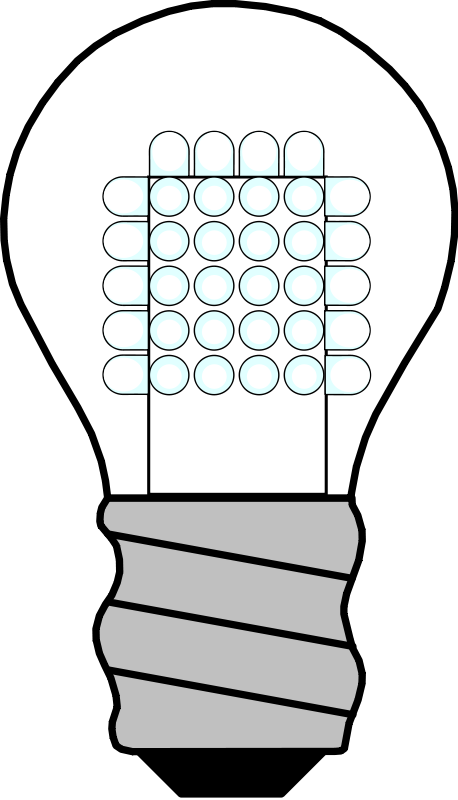
\includegraphics[scale=0.02]{imgs/bulb.png}
 \textbf{Nota} \\
 }%
{\endMakeFramed}

%Work in progress
\newenvironment{workinprogress}{%
  \def\FrameCommand{\colorbox{pink}}%
  \MakeFramed {\FrameRestore}
\lhdbend  \textbf{Work in progress} \\
 }%
{\endMakeFramed}

%Openquestion
\newenvironment{openquestion}{%
  \def\FrameCommand{\colorbox{pink}}%
  \MakeFramed {\FrameRestore}
 \textbf{Domanda aperta} \\
 }%
{\endMakeFramed}

%TODO
\newenvironment{todo}{%
  \def\FrameCommand{\colorbox{pink}}%
  \MakeFramed {\FrameRestore}
 \textbf{TODO} \\
 }%
{\endMakeFramed}

%%%%%%%%%%%%%%%%%%%%%%%%%%%%%%%%
%%%%%%%%%%%% HEADER %%%%%%%%%%%%
%%%%%%%%%%%%%%%%%%%%%%%%%%%%%%%%
\pagestyle{fancy}
% i comandi seguenti impediscono la scrittura in maiuscolo
% dei nomi dei capitoli e dei paragrafi nelle intestazioni
\renewcommand{\chaptermark}[1]{\markboth{#1}{}}
\renewcommand{\sectionmark}[1]{\markright{\thesection\ #1}}
\fancyhf{} % rimuove l'attuale contenuto dell'intestazione
% e del pi\`e di pagina
\fancyhead[LE,RO]{\bfseries\thepage}
\fancyhead[LO]{\bfseries\rightmark}
\fancyhead[RE]{\bfseries\leftmark}
\renewcommand{\headrulewidth}{0.5pt}
\renewcommand{\footrulewidth}{0pt}
\addtolength{\headheight}{0.5pt} % riserva spazio per la linea
\fancypagestyle{plain}{%
\fancyhead{} % ignora, nello stile plain, le intestazioni
\renewcommand{\headrulewidth}{0pt} % e la linea
}


%%%%%%%%%%%%%%%%%%%%%%%%%%%%%%%%
%%%%%%%%%%%% COLORS %%%%%%%%%%%%
%%%%%%%%%%%%%%%%%%%%%%%%%%%%%%%%
\definecolor{code}{gray}{0.3}


%%%%%%%%%%%%%%%%%%%%%%%%%%%%%%%%
%%%%%%%%%%%% NUMBERS %%%%%%%%%%%
%%%%%%%%%%%%%%%%%%%%%%%%%%%%%%%%
\setcounter{tocdepth}{3}
\setcounter{secnumdepth}{3}


%%%%%%%%%%%%%%%%%%%%%%%%%%%%%%%%
%%%%%%%%%%% DOC DATA %%%%%%%%%%%
%%%%%%%%%%%%%%%%%%%%%%%%%%%%%%%%
\title{Appunti di MNO}
\author{Gruppo Informatici Rampanti}
\date{ott 2010 - mag 2011}

\pdfinfo{%
  /Title    (Appunti di MNO)
  /Author   (Andrea Cimino e Lorenzo Muti)
  /Creator  (Andrea Cimino)
  /Producer (Lorenzo Muti)
  /Subject  (MNO)
  /Keywords (MNO)
}


%%%%%%%%%%%%%%%%%%%%%%%%%%%%%%%%
%%%%%%%%%%%%% UTILS %%%%%%%%%%%%
%%%%%%%%%%%%%%%%%%%%%%%%%%%%%%%%
% binary symbols
\newcommand{\modder}{\vdash _{R}}

% vertical gaps
\newcommand{\askip}{\vspace{0.5cm}}
\newcommand{\bskip}{\vspace{1.0cm}}

% various symbols
\newcommand{\qedhere}{\ensuremath{\Box}}
\newcommand{\qed}{\hfill \ensuremath{\Box}}

% substitution
\newcommand{\subst}[2]{^{#1} / _{#2}}

% denotational semantics function names
\newcommand{\bbracket}[1]{\left\llbracket #1 \right\rrbracket}

\newcommand{\aexpr}{\mathcal{A}}
\newcommand{\bexpr}{\mathcal{B}}
\newcommand{\cexpr}{\mathcal{C}}
\newcommand{\Aexpr}[1]{\mathcal{A} \bbracket{#1}}
\newcommand{\Bexpr}[1]{\mathcal{B} \bbracket{#1}}
\newcommand{\Cexpr}[1]{\mathcal{C} \bbracket{#1}}

\newcommand{\semdomset}[1]{(V_{#1})_{\bot}}

% semantic evaluations
\newcommand{\opereval}[3]{\left\langle #1, #2 \right\rangle \rightarrow #3}
\newcommand{\denaeval}[3]{\Aexpr{#1} #2 = #3}
\newcommand{\denbeval}[3]{\Bexpr{#1} #2 = #3}
\newcommand{\denceval}[3]{\Cexpr{#1} #2 = #3}

% rotated sqsubseteqs
\newcommand{\upsqsubseteq}{ $\begin{rotate}{90} $\sqsubseteq$ \end{rotate}$ }
\newcommand{\downsqsubseteq}{ $\begin{rotate}{270} $\sqsubseteq$ \end{rotate}$ }

% Space after paragraph declaration
\makeatletter
\renewcommand\paragraph{\@startsection{paragraph}{4}{\z@}%
  {-3.25ex\@plus -1ex \@minus -.2ex}%
  {1.5ex \@plus .2ex}%
  {\normalfont\normalsize\bfseries}}
\makeatother



% fast theorem and definition
\newcommand{\ftheo}[1]{\colorbox{YellowGreen}{#1}}
\newcommand{\fdefn}[1]{\colorbox{SkyBlue}{#1}}

\theoremstyle{break}
\theoremsymbol{\ensuremath{\clubsuit}}
\theoremseparator{\newline}
\newshadedtheorem{proc}[theo]{Procedura}

% bold math!
\newcommand{\bm}[1]{\mbox{\boldmath{$#1$}}}

\newcommand{\positive}[1]{\textbf{\color{green} +} #1}
\newcommand{\negative}[1]{\textbf{\color{red} -} #1}


\newtheoremlisttype{tab}%
{\begin{tabular*}{\linewidth}{@{}lrl@{\extracolsep{\fill}}r@{}}}%
{##1&##2&##3&##4\\}%
{\end{tabular*}}
\begin{document}
}
\providecommand{\outbpdocument}{\end{document}}
\else
\providecommand{\inbpdocument}{}
\providecommand{\outbpdocument}{}
\fi



\inbpdocument 

%% 5 Novembre (Bigi)
% \section{Bigi 5 nov}
\chapter{Richiami di Analisi e Ottimizzazione}
Vedremo Problemi di ottimizzazione:
 $$ f: \mathbb{R}^{n} \rightarrow \mathbb{R}, D \subseteq \mathbb{R}^{n}$$
  $$ \min \{ f(x) : x \in D \}$$
 Tovare $\overline{x} \in \mathbb{R}^{n}$ tale che
\begin{itemize}
 \item  $\overline{x} \in D$ (ammissibile)
 \item $f(\overline{x}) \leq f(x)$ per ogni $x \in D$ (punto di minimo)
\end{itemize}
Successione:
$$\{x_k\}_{k \in N} \subseteq \mathbb{R}^{n} \quad x_1,x_2,\ldots$$
Useremo la norma 2 su 
$\mathbb{R}^n$ :  $|| x ||_{2} = \sqrt{\displaystyle \sum_{i=1}^{r}x_{i}^2}$
\section{Richiami di analisi in $\mathbb{R}^{n}$}
\begin{defn}[Limite di una successione]
 $\overline{x} \in \mathbb{R}^n$ si dice limite di $\{ x_k \}_{k \in \mathbb{N}}$ 
se 
$$ \forall \varepsilon > 0 \; \exists  \overline{k} \quad \text{ t.c.} \quad  || x_k - \overline{x} ||_{2} \leq \varepsilon 
 \quad \forall k \geq \overline{k}$$
\end{defn}

\begin{example}
 $x_k = (1/k, 1/k)$ : il limite è il vettore $(0,0)$
\end{example}
Non tutte le successioni convergono
\begin{example}
 $x_k = ((1/k), (-1)^{k}) $: in questo caso il limite non esiste
\end{example}

\begin{defn}[Sottosuccessione]
 Selezione degli elementi $k_j$ tale che l'indice vada a $+\infty$.
\end{defn}
\begin{example}
Sottosuccessione $k_j = 2j-1$ ($k_j$ assume valori dispari)\\
Sottosuccessione $k_j = 2j$ ($k_j$ assume valori pari)
\end{example}
Nel caso dell'esempio, le singole sottosuccessioni definite convergono a
\begin{itemize}
 \item $(0,1)$
 \item $(0,-1)$
\end{itemize}
\begin{defn}[Punti di accumulazione della successione]
$\overline{x}$ è un punto di accumulazione di una successione
 $\{x_k\}$  se esiste una sottosequenza infinita di indici $k_j$ $ (k_1,k_2,
k_3, \ldots )$ tale che
$$\overline{x} =   \lim_{j \to +\infty}x_{k_{j}}$$

%$$ \lim_{n \to \infty}x_n	$$
\end{defn}

\begin{theo}[Bolzano-Weierstrass]
 Sia $\{x_k\}$ una successione tale che  esista una costante $M>0$ 
per cui $||x_k|| < M ~ \forall k$.\\
Allora $\{x_k\}$ ammette una sottosuccessione convergente.
\end{theo}

\begin{defn}[Insieme di vicini di $x$]
 Dato un punto $x \in \mathbb{R}^{n}$, chiamiamo
$\mathcal{N} \in \mathbb{R}^{n}$  \emph{insieme di vicini di x} se
è un insieme aperto che ccontiene $x$.
\end{defn}
Un insieme di vicini di $x$ molto utile è il seguente

\begin{defn}[Palla aperta di raggio $\varepsilon$ attorno a $x$]
Una palla aperta di raggio $\varepsilon$ attorno a $x$ \`e
definita come
$$ B(x,\varepsilon) = \{ y \; | \; ||y-x|| < \varepsilon \}$$
\end{defn}
In un piano bidimensionale abbiamo un cerchio.


\begin{defn}
 $A \subseteq \mathbb{R}^{n}$ si dice aperto se
$$\forall x \in A \quad \exists \varepsilon > 0 
   \text { t.c. }
 B(x, \varepsilon) \subseteq A
$$
\end{defn}

\begin{example}[Esempi di insiemi aperti]
  \begin{itemize}
  \item  $ ] -1, 1 [$
  \item $\mathbb{R}^{n}$
  \item $\emptyset$
  \end{itemize}
\end{example}

%% FIXME
\begin{property}
 unione di aperti è aperto
  $A_{\alpha} aperti \rightarrow \cup_{\alpha} A_{\alpha}$ è aperto
\end{property}
% {n \to \infty}

\begin{property}
\begin{itemize}
\item l'intersezione di un insieme finito di aperti è  un aperto
\item l'unione infinita di aperti è un aperto
\end{itemize}

\end{property}
L'intersezione infinita di $B(0, \frac{1}{k}) = \{0\}$ non è un aperto

\begin{defn}[Punto interno]
Sia $ A \subseteq \mathbb{R}^n$, $x$ si dice punto interno di $A$ se
$\exists \varepsilon > 0$ t.c. $B(x, \varepsilon) \subseteq A $
\end{defn}

\begin{property}
 $A$ aperto $\Longleftrightarrow ~ A=\{ \text{punti interni di  } A \}$
\end{property}

\begin{defn}[Chiuso]
$A \subseteq \mathbb{R}^{n}$ si dice \emph{chiuso} se
 $\mathbb{R}^{n} \backslash A$ (complementare) è aperto
\end{defn}

\begin{example}[Insiemi chiusi]
  \begin{itemize}
  \item $ \overline{B(x, \varepsilon) } = \{ y \in \mathbb{R}^{n} \; | \;\;  ||y-x||_{2} \leq \varepsilon \}$
  \item $\emptyset$
  \item $[-1,1]$
  \end{itemize}
\end{example}

\begin{defn}[Punto di chiusura] 
 Punto $x \in \mathbb{R}^{n}$ si dice \emph{punto di chiusura} se
 $$ \forall \varepsilon > 0: B(x, \varepsilon) \cap A \neq \emptyset $$
\end{defn}

\begin{property}
 A è chiuso $\Longleftrightarrow  A = \{ \text{punti di chiusura} \}$
\end{property}
Notazione:
$(\overline{A}, cl(A))$


\begin{property}
\begin{itemize}
 \item $A_{\alpha}$ chiusi $\Rightarrow$ $\cap_{\alpha} A_{\alpha}$ è chiuso.
  L'intersezione infinita di chiusi è un chiuso.
 \item $A_{i}$ chiusi $i=1 \ldots k \Rightarrow 
\displaystyle \bigcup_{i=1}^{k}A_{i}$ è chiuso.
L'unione finita di chiusi è un chiuso.
\end{itemize}

Ci sono per\`o degli elementi che possono essere sia aperti che chiusi e altri che non sono né aperti né chiusi \\
Gli insiemi vuoti e $\mathbb{R}^{n}$ sono sia aperti che chiusi.
\end{property}

\begin{example}[Insieme di elementi che non sono né aperti né
 chiusi]
 Prendiamo un rettangolo ed una palla (figura!)
 % FIXME aggiungere figura
$$([-1,0] \times [-1,1]) \cup B(0,1) = A$$
\begin{itemize}
\item 
   $(-1- \varepsilon, 0) \in B((-1,0),\varepsilon) \quad \forall \varepsilon$
   :  $A$ non è aperto
\item 
   $x_k = (1 - \frac{1}{k},0) \in A \quad x_k \rightarrow (1,0) 
 \notin A $: $A$ non è chiuso
\end{itemize}
\end{example}

\begin{property}
$A \subseteq \mathbb{R}^n $ è chiuso $\Longleftrightarrow
 \forall \{ x_k \} \subseteq A $ per cui $x_k  \rightarrow \overline{x}$
risulta $\overline{x} \in A $
\end{property}

\begin{defn}[Insieme limitato]
$A \subseteq \mathbb{R}^{n}$ si dice \emph{limitato}  se $\exists M > 0$ per cui
$|| x ||_{2} \leq M \; \forall x \in A $
\end{defn}

\begin{defn}[Insieme compatto]
 $A \subseteq \mathbb{R}^{n}$ si dice \emph{compatto} se A è limitato e chiuso.
\end{defn}
Gli insiemi compatti sono interessanti per il seguente motivo

\begin{theo}[Bolzano-Weirstrass]
\label{richiamibigi:bolzanow01}
 Sia $A \subseteq \mathbb{R}^{n}$ un insieme compatto.\\
 Ogni successione  $\{x_k\}_{k} \subseteq A$ ammette una sottosuccesione
 convergente.  Ossia
$$ \exists \{ x_{k_{j}}\} \subseteq A, \overline{x} \in A \text{ t.c. } x_{k_j} \rightarrow_{j \to + \infty} \overline{x}$$
\end{theo}

\subsection{Funzioni di pi\`u variabili a valori reali}%$f: \mathbb{R}^{n} \rightarrow \mathbb{R}}$

\begin{defn}[Funzione continua]
 $f$ si dice \emph{continua} in $\overline{x} \in \mathbb{R}^{n}$ se
 $$ \forall \varepsilon > 0 \quad \exists \delta > 0  \quad  \text{t.c.} \quad
\forall x \in \mathbb{R}^{n} : || x-\overline{x} ||_{2} \leq \delta  \Rightarrow | f(x) - f(\overline{x})| \leq \varepsilon $$ 
\end{defn}

\begin{property}
\label{richiamibigi:propfunzcont}
$f$ è continua in $\overline{x} \in \mathbb{R}^{n} \Longleftrightarrow
\forall \{x_k\}$ t.c. $x_k \rightarrow \overline{x}$ risulta 
$ \displaystyle \lim_{k \to +\infty}f(x_k) = f(\overline{x})$
\end{property}


\begin{example}[Esempi di funzioni continue]
  \begin{itemize}
  \item  $f(x) = || x ||_{2}$
  \item $f(x_1,x_2) = \sin(\pi x_1x_2)$
  \end{itemize}
\end{example}

\begin{defn}[Lipschitziana]
\label{def:lipschitziana}
Una funzione \emph{lipschitziana} è una funzione che ha una crescita
limitata, nel senso che il rapporto tra variazione di ordinata e
variazione di ascissa non può superare un valore fissato, detto
costante di Lipschitz. È una condizione più forte della continuità.
$$ \frac{||f(x_2) - f(x_1)||}{|| x_2 - x_1 ||} \leq L $$
\end{defn}


\begin{defn}[Estremo superiore]
Sia $(X,\leq)$ un insieme totalmente ordinato, $E\subseteq X$.
 Se esiste un elemento $y\in X$ tale che:
\begin{itemize}
\item $y$ è un maggiorante di $E$
\item se $z<y$ allora $z$ non è un maggiorante di $E$
\end{itemize}
diciamo che $y$ è \emph{estremo superiore} di $E$, in simboli
 $y=\sup E$ e diciamo che $E$ è limitato superiormente.
\end{defn}
La definizione di estremo inferiore è simmetrica.

\begin{defn}[Massimo]
Si definisce \emph{elemento massimo} di $S$  un elemento $M \in S$
 tale che
$$\forall a \in S,\ a\leq M$$
\end{defn}
La definizione di minimo è simmetrica.


\begin{theo}[Weirstrass per funzioni continue]
 Sia $A \subseteq \mathbb{R}^n$ compatto e
 $f: \mathbb{R}^{n} \rightarrow \mathbb{R}$ continua su $A$. \\
Allora $f$ ammette massimo e minimo su $A$.
\end{theo}

\begin{thproof}
Poniamo $ l = \inf \{f(x):  x \in A \} \in [ -\infty, + \infty]$.
Sicuramente esiste successione $f(x_k) \rightarrow l$ con $x_k \in A$. (per definizione di estremo inferiore). Ma
\begin{itemize}
\item Per la  (\ref{richiamibigi:bolzanow01}), $A$ compatto $\Rightarrow \exists x_{k_{j}} \rightarrow \overline{x}$

\item  Per la  (\ref{richiamibigi:propfunzcont})
$f$ continua $\Rightarrow  f(x_{k_{j}}) \rightarrow f(\overline{x})$ 
\end{itemize}
Allora, con l'unicità del limite,
 $f(\overline{x}) \Rightarrow l \neq -\infty \Rightarrow 
\min \{f(x): x \in A \}$

%  $x_k \in A $ $\{ x_k\} \subseteq A $
% $\{x_k\} \subseteq A$
% Per weirstrass
% $$x_{k_j} \rightarrow \overline{x} \in A $$
% Allora
% $$ f(\overline{x}) \leftarrow f(x_{k_j}) \rightarrow l$$
% Poiche il limite se esiste è unico
% $$f(\overline{x}) = l $$
\end{thproof}

\begin{example}
 $n = 1$  $f(t) = e^{-t}$, $A = \mathbb{R}_{+}$
 $$\inf \{ f(t): t \in A \} = 0$$ 
Ma il minimo non esiste! Quindi l'insieme non è compatto.
\end{example}

\subsection{Derivate}
Per le funzioni $f:\mathbb{R} \rightarrow \mathbb{R}$ abbiamo definito
la derivata come
$$ \lim_{t \to 0 } \frac{f(\overline{x} + t) - f(\overline{x})}{t}$$
Nel caso pi\`u generale di funzioni $f:\mathbb{R}^n \rightarrow \mathbb{R}^n$
consideriamo il punto $\overline{x}$ e l'insieme di vettori 
$$ \{ \overline{x} + tv \; | | \; t \geq 0  \} \quad  v \in \mathbb{R}^n, || v||_{2} = 1 \quad v:\text{direzione} $$

\begin{defn}[Derivata direzionale]
$f$ si dice \emph{derivabile in} $x \in \mathbb{R}^{n}$ 
\emph{nella direzione} $v$ se esiste
$$D_v f(\overline{x}) = \lim_{t \to 0 } \frac{f(\overline{x} + tv) - f(\overline{x})}{t}$$
\end{defn}

Le derivate direzionali sono una generalizzazione delle derivate
parziali, nelle quali si scelgono come vettori direzionali quelli
del tipo
$$ e_i = (0,0,0,\ldots, 0,\underbracket{1}_{\text{i-esima}},0, \ldots, \ldots, 0) $$
ecco una definizione più formale
\begin{defn}[Derivata parziale]
Si definisce derivata parziale di $f$ in $x$ rispetto alla variabile
$k-$esima $x_k$ il limite, se esiste finito
$$\frac{\partial f}{\partial x_k} (x)=\lim_{h\to 0}\frac{f(x_1,x_2,\ldots,x_k+h,\ldots,x_n)-f(x_1,x_2,\ldots,x_n)}{h}$$
\end{defn}

\begin{example}[Derivata parziale di $sin(\pi x_1 x_2)$]
\label{richiamibigi:example01}
$$f(x_1,x_2) = \sin(\pi x_1 x_2)  $$
Le 2 derivate parziali sono
$$
\frac{\partial f}{\partial x_1}(x) = \pi x_2 \cos(\pi x_1 x_2)
\qquad
\frac{\partial f}{\partial x_2}(x) = \pi x_1 \cos(\pi x_1 x_2)
$$
\end{example}

\begin{defn}[Gradiente]
$\nabla f(\overline{x}) = 
(\frac{\partial f}{\partial x_1}(\overline{x}),
\frac{\partial f}{\partial x_2}(\overline{x}),
\ldots,
\frac{\partial f}{\partial x_n}(\overline{x}))$
\`e detto \emph{gradiente} di $f$ in $\overline{x}$
\end{defn}
Informalmente, il gradiente indica la direzione di massima pendenza.\\
Nell'esempio (\ref{richiamibigi:example01}),  il vettore
$$ \nabla f(\overline{x}) = 
\begin{pmatrix}
  \pi x_2 \cos(\pi x_1 x_2) \\
\pi x_1 \cos(\pi x_1 x_2)
\end{pmatrix}
$$
i cui elementi sono le derivate parziali precedentemente calcolate,
è il \emph{gradiente di} $f$ \emph{in} $\overline{x}$.\\

%% 10 novembre
Prendiamo $ f: \mathbb{R}^{n} \rightarrow  \mathbb{R}$, $v \in \mathbb{R}^n$, $\Vert v \Vert = 1$

\begin{defn}[Two-sided derivate]
$$\dfrac{\partial f}{\partial v}(\overline{x}) = \lim_{t \to 0} \dfrac{[f(\overline{x}+t \cdot v)-f(\overline{x})]}{t}$$
\end{defn}

\begin{defn}[One-sided directional derivate]
$$f'(\overline{x}, v) = \lim_{t \to 0^{+}} \dfrac{[f(\overline{x}+t \cdot v)-f(\overline{x})]}{t}$$
Il limite invece che andare a $0$ da entrambi i lati, ci va solo da $0^+$.
\end{defn}

\begin{notes}
A volte esiste una e non l'altra.
\end{notes}

\begin{example}[Derivate della norma]
 $$f(x) = || x ||_2 = ( \displaystyle \sum_{i=1}^{n} x_i^2)^{1/2} \quad
 v \in \mathbb{R}^{n} \quad ||v||_{2} = 1 \quad, \overline{x} = 0
 $$
$$  \frac{f(\overline{x} + tv) - f(\overline{x})}{t} = \frac{f(tv)}{t} = 
\frac{( \displaystyle \sum_{i=1}^{n} t^{2}v_{i}^{2})^{1/2}}{t} = 
\frac{|t| (\displaystyle \sum_{i=1}^{n} v_i^{2})^{1/2}}{t} =sgn(t) ||v||_{2} = sgn(t) 
$$
Quindi $f'(\overline{x}, v) = 1$ mentre $\dfrac{\partial f}{\partial v}(\overline{x})$ non esiste.
\end{example}

\begin{example}[Esempi di calcolo di derivata in $\mathbb{R}^{n}$]
Prendiamo ad esempio la funzione $f$ definita nel seguente modo
\begin{equation}
\label{richiamibigi:example01}
f(x_1,x_2) =
\begin{cases}
\left(\frac{x_1^2 x_2}{x_1^4+x_2^2}\right)^2 & \text{ se } (x_1,x_2) \neq (0,0)\\
indef. & \text{ se } (x_1,x_2) = (0,0)
\end{cases}
\end{equation}

Ponendo  $x_2 = \alpha x_1^2,$  risulta
$$f(x_1, \alpha x_1^2) = \left[\alpha x_1^4 \cdot (x_1^4 + \alpha^2 x_1^4 ) \right]^2 = \left[\alpha / (1+ \alpha^2 ) \right]^2$$
% \cdots ~ \mbox{$f$ non è continua.}
% $$

\begin{openquestion}
  Perch\`e ha voluto introdurre questo $\alpha$?
  Voleva mostrare qualcosa in particolare?
\end{openquestion}

$f$ risulta non continua in $\overline{x} = (0,0)$.
Consideriamo infatti le seguenti successioni:

\begin{itemize}
\item $f(\frac{1}{k}, \frac{1}{k^2})$. Sostituendo i parametri
  in (\ref{richiamibigi:example01}) otteniamo il valore costante
  $1/4$.\\
 Per $k \to +\infty$ la successione converge a $(0,0)$ , ma risulta
 $$ \lim_{ k \to \infty} f\left(\frac{1}{k}, \frac{1}{k^2}\right) = 1/4
     \quad \neq \quad 
     ? = f(\overline{x})
 $$
\item $f(\frac{1}{k}, \frac{2}{k^2})$: discorso analogo al caso precedente.
Risulta infatti $f(\frac{1}{k}, \frac{2}{k^2}) = 4/25$, ma
 $$ \lim_{ k \to \infty} f\left(\frac{1}{k}, \frac{2}{k^2}\right) = 4/25
 \quad \neq \quad 
? = f(\overline{x})
$$
\end{itemize}

\begin{openquestion}
Perch\`e ha mostrato due esempi? Non ne bastava solo uno per
provare la non continuit\`a?
\end{openquestion}
Facciamo vedere che esistono le derivate direzionali di $f$
in $\overline{x}=(0,0)$ in tutte le direzioni. Ricordiamo
che $x$ e $v$ sono vettori e $t$ \`e uno scalare.
Poniamo $f(\overline{x}) = 0$.
$$
\begin{array}{c}
\displaystyle \frac{\partial f}{\partial v}(\overline{x})=
\displaystyle \frac{\partial f}{\partial v}((0,0))=
\displaystyle  \lim_{t \to 0}
\dfrac{f\left(\left(0,0 \right) + t\left(v_1,v_2 \right) \right) - 
\overbracket{f((0,0))}^{0}}{t} = \\
\displaystyle  \lim_{t \to 0}
 \dfrac{f \left(\left(tv_1,tv_2 \right) \right)}{t} =
\displaystyle  \lim_{t \to 0}\frac{[t^3 v_1^2 v_2 /(t^4 v_1^4 + t^2 v_2^2)]^2}{t} 
= \displaystyle \lim_{t \to 0} t v_1^{4} v_2^{2} / (t^2 v_1^4 + v_2^2)^2 
  \xrightarrow{t \to 0} 0
\end{array}
$$
\end{example}
Dall'esempio precedente abbiamo stabilito qundi che la propriet\`a:
$$ 
\varphi: \mathbb{R} \rightarrow \mathbb{R},  \qquad 
\varphi \text{ derivabile in } \overline{x}
\quad
\Longrightarrow
\quad
\varphi \text{ continua in } \overline{x}
$$
non vale in generale in $\mathbb{R}^{n}$.

\begin{notes}
Le derivate in tutte le direzioni esistono, quindi non è come nelle
equazioni ad una variabile: se $f$ è derivabile, non è 
necessariamente continua.
\end{notes}


\begin{defn}[Funzione lineare]
Una funzione $L$ è lineare se e solo se
$$
x,y \in \mathbb{R}^n  \quad  \alpha,  \beta \in \mathbb{R}
\qquad L(\alpha x + \beta y) = \alpha \cdot L(x) + \beta \cdot L(y) 
$$
ovvero:
$$
L(x) = l^T x = \sum_{i=1}^{n}l_i x_i
$$
\end{defn}

\begin{defn}[Funzione differenziabile]
$f: \mathbb{R}^n \to \mathbb{R}$ si dice \emph{differenziabile} 
in $\overline{x} \in \mathbb{R}^n$ se $\exists ~ L: \mathbb{R}^n \to \mathbb{R}$
lineare tale che
$$\forall h \in \mathbb{R}^n 
\quad 
 f(\overline{x}+h)=f(\overline{x}) + L(h) + r_{\overline{x}}(h)$$
con $r_{\overline{x}}(h)$ un resto tale che  $\dfrac{r_{\overline{x}}(h)}{\Vert h\Vert_2} \to 0 $ per  $ \Vert h\Vert_2 \to 0$
\end{defn}

\begin{openquestion}
 Mi sembra di aver capito che una funzione differenziabile
implica che tutte le derivate, da tutte le direzioni, sono
esprimibili come combinazione lineare delle derivate della
base canonica. La cosa verr\`a esplicitata nell'esercizio
(\ref{richiamibigi:exercise01})
\end{openquestion}
In altri termini, la differenza tra la funzione in un punto e la
funzione calcolata in $\overline{x}$ è approssimata da una funzione lineare.

\begin{property}
Sia $f:\mathbb{R}^n \rightarrow \mathbb{R}$

$f$ differenziabile in $\overline{x} \quad \Longrightarrow \quad f$
 continua in $\overline{x}$
\end{property}
 
\begin{notes}
(Quest'ultima proprietà è simile a quella delle funzioni a una variabile)  
\end{notes}

\begin{property}
\label{richiamibigi:diffimpliesderivatives}
Sia $f:\mathbb{R}^n \rightarrow \mathbb{R}$

$f$ differenziabile in $\overline{x} 
\quad \Longrightarrow \quad f$ ammette derivate in $\overline{x}$ in ogni
direzione $v$.
\end{property} 

\begin{thproof}
$$
\begin{array}{c}
 \dfrac{\partial f}{\partial v}(\overline{x}) = 
 \displaystyle
 \lim_{t \to 0} \dfrac{f(\overline{x}+ tv) - f(\overline{x})}{t} =
 \lim_{t \to 0} \dfrac{L(tv)+ r_{\overline{x}}(tv)}{t} =
 \lim_{t \to 0} \dfrac{tL(v)+ r_{\overline{x}}(tv)}{t} =
 L(v) + \lim_{t \to 0}  \dfrac{r_{\overline{x}}(tv)}{t} = L(v) \\ \\

\Vert tv \Vert_2 = t \Vert v \Vert_2 = t
\end{array}
$$
(Nota che $\Vert v \Vert_2 = 1$)
\end{thproof}

\begin{openquestion}
Da quello che ho capito dalle note
una volta stabilito che  \\
$f$ differenziabile in $\overline{x} 
\quad \Longrightarrow \quad f$ ammette 
derivate in $\overline{x}$ in ogni direzione $v$.
\\Si vuole avere un metodo esplicito per calcolare
la derivata direzionale. Chiedere lumi.
A occhio mi viene da dire che, una volta calcolate le derivate
parziali della base canonica, possiamo ricavare le derivate
delle direzioni facendo un semplice prodotto riga per colonna.
La condizione che deve essere rispettata \`e che $f$ deve
essere differenziabile.
\end{openquestion}

\begin{observation}[Calcolo esplicito della derivata direzionale]
Sfruttiamo le seguenti ipotesi:
$$v \in \mathbb{R}^n \qquad \Vert v \Vert_2 = 1 
    \qquad  v=\sum_{i=1}^{n}v_i  e_i 
\qquad \underbracket{f \text{ differenziabile}}_{\text{CHECKME}}
$$
calcoliamo quindi la  derivata direzionale
$$
\frac{\partial f}{\partial v}(\overline{x}) =
 L(v) =
 L \left( \sum_{i=1}^n v_i  e_i \right)
 \; \underbracket{=}_{1)}  \;
  \sum_{i=1}^n v_i \cdot L(e_i) = 
  \sum_{i=1}^n v_i \frac{\partial f}{\partial x_i}(\overline{x})  =
   \nabla f (\overline{x})^T v $$
  \begin{enumerate}
  \item $L$ è lineare
  \end{enumerate}
\end{observation}

\begin{exercise}
\label{richiamibigi:exercise01}
Esercizio per casa: studia
$$
   f(x_1, x_2)= \begin{cases}x_1^2 x_2 / (x_1^2 + x_2^2)  
    & \mbox{se } (x_1, x_2) \neq (0,0)  \\
   0 & \mbox{se } (x_1,x_2) = (0,0)\end{cases}
$$
\textbf{Svolgimento} \\
Vediamo che questa funzione non \`e differenziabile in
$\overline{x} = (0,0)$
$$
\dfrac{\partial f}{\partial v} (\overline{x})
=
\lim_{t \to 0}
\dfrac{t^{3}v_1^{2}v_2 / t^{2}(\overbracket{v_1^{2} + v_2^{2}}^{||v||_2^{2}})}{t}
=
v_1^{2}v_2
 \qquad ( \text{poich\`e } ||v||_{2}^{2} = v_1^{2} + v_2^{2} = 1)
$$
In particolare abbiamo
$$\dfrac{\partial f}{\partial x_1} (\overline{x})
=
\dfrac{\partial f}{\partial x_2} (\overline{x})
=
0
$$
Per farlo vedere, specialmente in questa fase iniziale del corso,
eplicitiamo i conti:
$$\dfrac{\partial f}{\partial x_1} (\overline{x}) =
1^{2}\cdot 0  = 0
$$ 
Nell'altro caso
$$\dfrac{\partial f}{\partial x_2} (\overline{x}) =
0^{2}\cdot 1  = 0
$$ 
ma $\dfrac{\partial f}{\partial v} (\overline{x}) \neq 0$
per ogni altra direzione. Quindi
$
\dfrac{\partial f}{\partial v} (\overline{x})
\neq
\nabla f(x)^{T}v = 0
$ \\
\begin{openquestion}
\`E vero che il motivo profondo della disuguaglianza \`e che la derivata
in ogni direzione non \`e esprimibile come combinazione
lineare delle derivate perziali sulle direzioni della base canonica?
\end{openquestion}
\end{exercise}

\begin{theo}[Differenziale totale]
\label{richiamibigi:differenzialetotale}
Sia $f:\mathbb{R}^n \to \mathbb{R}$, tale da ammettere derivate
parziali in ogni $x \in B(\overline{x},\varepsilon)$ per qualche
$\varepsilon > 0$. Allora
$$
\frac{\partial f}{\partial x_i}: B(\overline{x}, \varepsilon)
 \to \mathbb{R}  \text{  continua in  } \overline{x}
\quad  \Longrightarrow \quad f  \text{  differenziabile in  }
 \overline{x}
$$

$$f \to \frac{\partial f}{\partial x_i}(\overline{x})$$
\end{theo}

\begin{example}
Vediamo un'applicazione pratica del teorema
 (\ref{richiamibigi:differenzialetotale}) appena enunciato. 
Dalla tabella di verit\`a delle implicazioni  possiamo stabilire 
che vale la propriet\`a
$$
 (a \; \Longrightarrow \; b ) \quad
\Longleftrightarrow \quad
(\neg b \; \Longrightarrow \;  \neg a )
$$

Facciamo vedere quindi che non derivabilit\`a implica
non continuit\`a. \\
Riprendiamo l'esercizio (\ref{richiamibigi:exercise01}):
$$
\begin{array}{c}
\dfrac{\partial f}{\partial x_1}(x) =
\underbracket{D(x_1^2 x_2 / (x_1^2 + x_2^2))}_{\text{rispetto a } x_1} 
\underbracket{=}_{1)}
\dfrac{
D(x_1^2 x_2 ) (x_1^2 + x_2^2) 
-
x_1^2 x_2  D(x_1^2 + x_2^2) 
} { (x_1^2 + x_2^2)^{2}} =   \\
 \dfrac{ \cancel{2x_1 x_2^{3}}
+2x_2^{3} x_1   \cancel{ - 2x_1 x_2^{3}}
}{(x_1^{2} + x_2^{2})^{2}} 
=
\dfrac{2x_2^{3} x_1 }{(x_1^{2} + x_2^{2})^{2}} 
\end{array}
$$
\begin{enumerate}
\item Derivata del rapporto
\end{enumerate}
Ponendo $x_1 = x_2 = k$, $k \neq 0$ otteniamo
$$
\dfrac{\partial f}{\partial x_1}(x_1,x_2) =
\dfrac{2k^{4}}{(2k^{2})^{2}} = \dfrac{1}{2}$$ 

Mentre, come visto precedentemente nell'esempio
$$\dfrac{\partial f}{\partial x_1}(0,0) = 0$$
\end{example}

\begin{property}[Funzioni composte]
Sia
$f\; : \; \mathbb{R}^n \to \mathbb{R}$  differenziabile in
$ \overline{x} \in \mathbb{R}^n$,
$\Phi \; : \;  \mathbb{R} \to \mathbb{R} $ derivabile in 
$f(\overline{x}) \in \mathbb{R}^n$. \\
Allora
$\Phi \circ f:\mathbb{R}^n \to \mathbb{R}$ è differenziabile in 
$\overline{x}$ con

$$  \nabla(\Phi \circ f)(\overline{x}) = 
\Phi'(f(\overline{x})) \nabla f(\overline{x})$$
\end{property}

\begin{theo}[Valor medio]
$f:\mathbb{R}^n \to \mathbb{R}$ è differenziabile (su tutto $\mathbb{R}^n$)
con continuità (cioè $x \mapsto \nabla f(x)$ è continua)
su $\mathbb{R}^{n}$. \\
Dati $\overline{x}, h \in \mathbb{R}^n$, esiste $t \in (0,1)$ t.c.
 $$f(\overline{x}+h) = f(\overline{x}) + \nabla f(\overline{x} + th)^T h$$
\end{theo}

\begin{notes}
Notare che $x + th$ appartiene al segmento di estremi $x$ e $x+h$.
Ricordare inoltre il caso
$$  \Phi : \mathbb{R} \rightarrow \mathbb{R}\; : \;
\Phi(t_1) = \Phi(t_0) +   \Phi'(\xi)(t_1 -t_1)
\text{ per un opportuno } \xi
\in (t_1, t_0)
(t_0,t_1) 
$$
\end{notes}

\begin{defn}[Formula di Taylor del 1$^o$ Ordine]
Sia $f:\mathbb{R}^{n} \rightarrow \mathbb{R}$ differenziabile, allora la formula
di Taylor del primo ordine risulta
$$ 
f(\overline{x} + h) =
 f(\overline{x}) + \nabla f (\overline{x})^T h + r(h)
\qquad \text{ con  }\; 
\dfrac{r(h)}{||h||_{2}} \xrightarrow{ || h ||_{2} \to 0} 0$$
\end{defn}
Quest'ultima \`e una semplice riscrittura della definizione
alla luce della propriet\`a (\ref{richiamibigi:diffimpliesderivatives}) 

\begin{defn}[Iperpiano tangente]
$h = x - \overline{x}$, $h \approx 0  
\rightarrow f(x) \approx f(\overline{x})
 + \nabla f(\overline{x}^{T}(x - \overline{x})$
\\
Equazione iperpiano tangente al grafico di $f$ nel punto
 $(\overline{x}, f(\overline{x}))$
$$ \left\{ (x, f(\overline{x}) + \nabla f(\overline{x})^{T}(x-\overline{x})) 
\; | \; x \in \mathbb{R}^{n} \right\}$$
\end{defn}


\subsubsection{Derivate seconde}
$$
\begin{array}c
f:\mathbb{R}^n \to \mathbb{R} ~ \mbox{differenziabile}\\
x \to \dfrac{\partial f}{\partial v}(x) \qquad \dfrac{\partial f}{\partial v}: \mathbb{R}^n \to \mathbb{R}\\
\overline{x} \in \mathbb{R}^n, \quad v \in \mathbb{R}^n, \quad \Vert v \Vert_2 = 1, \quad w \in \mathbb{R}^n, \quad \Vert w \Vert_2 = 1\\
\dfrac{\partial}{\partial w}\left(\dfrac{\partial f}{\partial v} \right)(\overline{x}) = \lim_{t \to o}\dfrac{\frac{\partial f}{\partial v}(\overline{x} + tw)-\frac{\partial f}{\partial v}(\overline{x})}{t}\\
w = e_1, \quad v = e_j\\
\dfrac{\partial}{\partial x_1}\left(\dfrac{\partial f}{\partial x_2}\right) \underbrace{\longrightarrow}_{\mbox{si scrive}} \dfrac{\partial^2 f}{\partial x_1 \partial x_2}
\end{array}
$$  

Esercizio: $f(x_1, x_2)= sin(\pi x_1 x_2)$ calcolare le 4 derivate parziali.

\subsection{Funzioni  di pi\`u variabili a valori vettoriali}%$\mathbb{R}^{n} \rightarrow  \mathbb{R}^{n}$}
%% 12 Novembre
\begin{defn}[Matrice Jacobiana]
$F: \mathbb{R}^{n} \rightarrow \mathbb{R}^{n} \quad
F=(f_1,\ldots, f_n)$ \\
Matrice dei gradienti: righe sono i gradienti.
$$ J_{F}(x) =
\begin{pmatrix}
\nabla f_1(x)^{T} \\
 \nabla f_2(x)^{T} \\
 \ldots \\
\nabla f_n(x)^{T} 
\end{pmatrix} =
\begin{pmatrix}
\frac{{\partial} f_1(x)}{{\partial}(x_1)}(x) & \ldots &  \frac{{\partial} f_1(x)}{{\partial}(x_n)}(x)\\
 \ldots & \ldots & \ldots \\
\frac{{\partial} f_n(x)}{{\partial}(x_1)}(x) & \ldots &  \frac{{\partial} f_n(x)}{{\partial}(x_n)}(x)
% \frac{{\partial} f_n(x)}{{\partial}(x_1)}(x} ....  \frac{{\partial} f_n(x)}{{\partial}(x_n(}(x}
\end{pmatrix}
$$
\end{defn}
Il determinante della matrice Jacobiana \`e detto Jacobiano.

\subsection{Derivate di ordine superiore}
$f$ differenziabile su $\mathbb{R}^{n} 
\quad 
\Rightarrow
\quad 
\exists
\dfrac{\partial f }{\partial v}(x)
$
per ogni $x \in \mathbb{R}^{n}$, $v\in \mathbb{R}^{n}$ con 
$||v||_2 =1$ . \\
$\dfrac{\partial f }{\partial v}:
\mathbb{R}^{n} \rightarrow \mathbb{R}$ \`e una funzione
$\rightarrow$ ammette derivate nelle varie direzioni? \\
Limitiamoci alle derivate parziali: $w=e_i, v=e_j
\quad \rightarrow \quad
\dfrac{\partial}{\partial x_j} \rightsquigarrow
\dfrac{\partial^{2}f}{\partial x_i \partial x_j}
\quad
i=j \rightsquigarrow \dfrac{\partial^{2}f}{\partial x_i^{2}}
$

Funzioni  $\mathbb{R}^{n} \rightarrow  \mathbb{R}$ differenziabile:
$$\frac{{\partial} f}{{\partial}(x_j)}: \mathbb{R}^n \rightarrow \mathbb{R}$$
%%FIXME
\begin{example}
Definiamo $f$ come $ f(x_1,x_2) = \sin(\pi x_1 x_2)$
$$
\begin{array}{l}
\frac{{\partial}} {{\partial}(x_1)}f(x) = \pi x_2\cos(\pi x_1 x_2) \\
\frac{{\partial}} {{\partial}(x_2)}f(x) = \pi x_1\cos(\pi x_1 x_2)  \\

\frac{{\partial}^2 f} {{\partial} x_2 {\partial} x_1}(x) = \pi 
\cos(\pi x_1 x_2) - \pi^2 x_2 x_1 \sin(\pi x_1 x_2)       \\
\frac{{\partial}^2 f} {{\partial} x_1 {\partial} x_2}(x) 
= \pi \cos(\pi x_1 x_2) - \pi^2 x_1 x_2 \sin(\pi x_1 x_2) \\
\end{array}
$$
Le due derivate parziali sono uguali.
Scambiando l'ordine di derivazione abbiamo ottenuto lo stesso
risultato: non è un caso, deriva dal seguente teorema.
\end{example}
\begin{theo}[Schwarz/inversione ordine di derivazione]
\label{th:schwarz}
 Sia $f: \mathbb{R}^n \rightarrow \mathbb{R}$ tale che per ogni $i,j = 1\ldots n$
tali che
$\frac{{\partial}^2 f}{{\partial} x_j {\partial} x_i} \; ,\; \frac{{\partial}^2 f}{{\partial} x_i {\partial} x_j}$
esistano in $B(\overline{x}, \varepsilon)$ per $\overline{x} \in \mathbb{R}^n, \varepsilon > 0$ e siano continue in $\overline{x}$.
Allora:
$$\frac{{\partial}^2 f}{{\partial} x_j {\partial} x_i} =  \frac{{\partial}^2 f}{{\partial} x_i {\partial} x_j}$$
\end{theo}
\begin{defn}[Matrice Hessiana di $f$ in $f: \mathbb{R}^n \rightarrow \mathbb{R}$ in $\overline{x} \in \mathbb{R}^n$]
$$ \nabla^2 f(\overline{x}) = \left\{ 
 \frac{{\partial}^2 f}{{\partial} x_i {\partial} x_j}
  \right\}_{\substack{i=1 \ldots n \\j=1\ldots n}} = 
\begin{pmatrix}
\dfrac{{\partial}^2 f}{{\partial} x_1^2}(\overline{x}) & 
\dfrac{{\partial}^2 f}{{\partial} x_1 \partial x_2}(\overline{x}) & \ldots &
   \dfrac{{\partial}^2 f}{{\partial} x_1{\partial} x_n }(\overline{x}) \\
 \vdots   & \vdots  & \vdots & \vdots   \\
 \vdots   & \vdots  & \vdots  & \vdots   \\
\dfrac{{\partial}^2 f}{{\partial} x_n{\partial} x_1 }(\overline{x})
 & \ldots & \ldots &  \dfrac{{\partial}^2 f}{{\partial} x_n{\partial} x_n }(\overline{x})
\end{pmatrix}
$$
\end{defn}
Differenziabile due volte
$\frac{{\partial}^2 f}{{\partial} x_i {\partial} x_j}(x)$ esista per ogni $x \in \mathbb{R}^{n}$
e 
$\frac{{\partial}^2 f}{{\partial} x_i {\partial} x_j}: \mathbb{R}^n \rightarrow \mathbb{R}  $
sia continua su $\mathbb{R}^n$.
Questa è una matrice \emph{simmetrica}

\begin{defn}[Formula di Taylor con resto]
 $$f(\overline{\mathbf{x}}+\mathbf{h}) = f(\overline{\mathbf{x}}) +
 \nabla f(\overline{\mathbf{x}})^T\mathbf{h} + 
 \frac{1}{2}  \mathbf{h}^T \nabla^{2} f(\overline{\mathbf{x}} +
 t  \mathbf{h}) \mathbf{h}
\qquad
\text{con } t \in (0,1) \text{ opportuno}
$$
\end{defn}

\begin{defn}[Formula di Taylor secondo ordine]
 $$f(\overline{\mathbf{x}}+\mathbf{h}) = 
f(\overline{\mathbf{x}}) +
 \nabla f(\overline{\mathbf{x}})^T\mathbf{h} + 
 \frac{1}{2} 
\underbracket{ \mathbf{h}^T \nabla^{2} f(\overline{\mathbf{x}}) \mathbf{h}}_{}
+ r_{\overline{x}}(h)
\qquad
\text{con } \dfrac{r_{\overline{\mathbf{x}}}(\mathbf{h})}{||\mathbf{h}||_{2}^{2}}
\xrightarrow{||\mathbf{h}||_{2} \to 0} 0
$$

$$\mathbf{h}^{T} \nabla^{2} f(\overline{\mathbf{x}}) \mathbf{h} =
 \displaystyle \sum_{i=1}^{n} \displaystyle \sum_{j=1}^{n}
 = \frac{{\partial}^2 f}
{{\partial} x_i {\partial} x_j}
(\overline{\mathbf{x}}) h_i h_j$$
\end{defn}
Questa formula è interssante quando $h$ è piccolo, infatti
$$ 
\mathbf{h} = \mathbf{x} - \overline{\mathbf{x}} \approx 0
\; : \;
f(\mathbf{x}) \approx
\underbracket{ f(\overline{\mathbf{x}}) + \nabla f(\overline{\mathbf{x}})^{T} (\mathbf{x}-\overline{\mathbf{x}}) + 
 \underbracket{\frac{1}{2}(\mathbf{x}- \overline{\mathbf{x}})^{T}\nabla^{2} f(\overline{\mathbf{x}})(\mathbf{x}-\overline{\mathbf{x}})}_{\text{funzione non lineare}}}_{\text{approssimazione quadratica di} f  \text{ vicino a } \mathbf{x}} $$

Funzioni alle quali saremo molto interessanti sono le funzioni quadratiche
\begin{defn}[Funzione Quadratica]
Siano $ Q \in \mathbb{R}^{n \times n}, b \in \mathbb{R}^{n}, c \in \mathbb{R} $.
La funzione: $f: \mathbb{R}^{n} \rightarrow \mathbb{R}$ \`e detta
\emph{funzione quadratica} se 
 $$ 
f(x) =  \frac{1}{2} x^{T} Q x + b^{T}x + c 
=
\frac{1}{2} 
 \displaystyle \sum_{k=1}^{n} \displaystyle \sum_{l=1}^{n}
q_{kl} x_{k}x_{l} + \displaystyle \sum_{k=1}^{n} b_k x_k + c
$$
\end{defn}

\begin{notes}
Una forma quadratica \`e una funzione quadratica in cui
sono presenti solo i termini di secondo grado, ossia
$$f(x) =  \frac{1}{2} x^{T} Q x $$
\end{notes}
et{=}_{\text{simmetrica}}
\label{obs:gradiente-hessiana-funzione-quadratica}
Cosa accade se $Q$ \`e simmetrica in una funzione lineare?
Valgono le seguenti propriet\`a:
\begin{enumerate}
\item (Gradiente): $\nabla f(x) = Qx + b$
\item(Matrice Hessiana): $\nabla^{2}f(x) = Q$
\end{enumerate}
 % : $q_{kl}$ : $q_{kl} \rightsquigarrow (q_{kl} + q_{lk})/2$
% Si potrebbe pensare che questa  matrice $Q$ sia simmetrica 
% Facendo i conti:\\ 
% Gradiente di $f(x) = Qx + b$\\
% Matrice Hessiana: $Q$\\
Dimostriamo 1. Vediamo cosa vale la derivata parziale in una generica
componente $j$
$$
\begin{array}{c}
\dfrac{\partial f}{\partial x_j}(x) =
\dfrac{1}{2}
\left[\displaystyle \sum_{l=1}^{n} q_{jl}x_l 
+
\sum_{k=1}^{n} q_{kj}x_k
\right] + b_j \underbracket{=}_{\text{simmetrica}}
\dfrac{1}{2}
\left[\displaystyle \sum_{l=1}^{n} q_{lj}x_l 
+
\sum_{k=1}^{n} q_{kj}x_k
\right] + b_j = \\
\displaystyle \sum_{l=1}^{n} q_{jl}x_l + b_j =
(Qx)_j + b_j  \qquad \Longrightarrow \qquad 
\nabla f(x) = Qx + b
\end{array}
$$
Discorso analogo per il punto 2.
$$
\dfrac{\partial f}{\partial x_i \partial x_j}(x) 
= 
\dfrac{\partial f}{\partial x_i}
\left(\dfrac{\partial f}{\partial x_j}(x) 
\right)
=
\dfrac{\partial f}{\partial x_i}
\left(
\displaystyle \sum_{l=1}^{n} q_{jl} x_{l} + b_j 
\right) = q_{ji} = q_{ij}
\qquad \Longrightarrow \qquad \nabla^{2}f(x) = Q
$$
%\end{observation}

\begin{exercise}
Per esercizio :
trovare l'approssimazione di Taylor del secondo
ordine di
 $f(x_1,x_2) = - x_1^4 -x_2^2$ centrata in $\overline{x} = (0, 2/5)$
 \\
\textbf{Svolgimento}
$$
\nabla f(x) = 
\begin{pmatrix}
  -4 x_1^{3} \\
  -2 x_2
\end{pmatrix}
\qquad
\nabla^{2} f(x) = 
\begin{pmatrix}
  -12 x_1^{2} & 0 \\
  0 & -2
\end{pmatrix}
$$

$$
\overline{x} = (0, 2/5)
\qquad
\nabla f(\overline{x}) = 
\begin{pmatrix}
   0  \\
  -4/5
\end{pmatrix}
\qquad
\nabla^{2} f(\overline{x}) = 
\begin{pmatrix}
  0 & 0 \\
  0 & -2
\end{pmatrix}
$$

$$
\begin{array}{l}
f(\overline{x} +h) = f(\overline{x}) +
  \nabla f(\overline{x})^{T}(x- \overline{x})
  + \dfrac{1}{2}( x - \overline{x})^{T}
   \nabla^{2} f(\overline{x}) (x - \overline{x}) = \\
-\dfrac{4}{25} - \dfrac{4}{5} (x_2 + \dfrac{2}{5}) 
   - 2(x_2 + \dfrac{2}{5}x)^{2} = \\
-\dfrac{12}{25} -\dfrac{4}{5} x^{2} - 2x_2^{2} - 
   \dfrac{8}{25} - \dfrac{8}{5} x^{2} = \\
   \dfrac{20}{25} - \dfrac{12}{5} x_2 - 2x_2^{2} 
\end{array}
$$

\begin{todo}
 Magari mettere un bel grafico 3d per evidenziare
il comportamento di Taylor. 
\end{todo}
\end{exercise}

\chapter{Ottimizzazione: regione ammissibile e condizioni di ottimalità}
\label{chap:ottimizzazioni-definizioni}
\begin{todo}
Dare un nome pi\`u sensato al capitolo ed alle sezioni.
\end{todo}
$ f: \mathbb{R}^n \rightarrow \mathbb{R}, D \subseteq \mathbb{R}^n$\\
$$\text{(P)} \qquad
\min\{ f(x)\; : \; x \in D \}
$$

Problema: trovare $\overline{x} \in \mathbb{R}^n $ tale che:

\begin{itemize}
 \item $\overline{x} \in D$
 \item $f(\overline{x}) \leq f(x) \; \forall x \in D$
\end{itemize}

\paragraph{Classificazione della regione ammissibile}
$$
\left\{
\begin{array}{ll}
 D = \mathbb{R}^{n} &      \text{ Ottimizzazione  non vincolata } \\
 D \subset \mathbb{R}^n & \text{ Ottimizzazione  vincolata } 
\end{array}
\right.
$$
%Ottimizzazione sul continuo e sul discreto.

\paragraph{Classificazione della funzione obiettivo}
$$f \text{ obiettivo}: \left\{
\begin{array}{l}
 \text{lineare} \\
 \text{non lineare}
\end{array}
\right.
$$
\begin{defn}[Punto di minimo globale]
$\overline{x} \in \mathbb{R}$ si dice 
\emph{punto di minimo globale} di (P) se
\begin{itemize}
\item $x \in D$
\item $f(\overline{x}) \leq f(x) \quad
\forall x \in D$
\end{itemize}
\end{defn}
In questo caso $f(\overline{x})$ si dice
\emph{valore ottimo} di (P)
\begin{observation}
 Punto di minimo e inf non sono la stessa cosa! \\

 Ad esempio $f(x) = e^{-x}$ ha estremo inferiore ma 
non ha minimo.Quindi possiamo afferemare che il valore
ottimo esiste (inteso come $inf\{f(x)\; : \; x \in D \}$),
ma non esiste alcun cun punti di minimo. \\
Prendiamo invece la funzione
$f(x) = -x^{2}$: il valore ottimo non esiste in quanto
$f(x) \rightarrow -\infty$.
\end{observation}
\begin{figure}[h]
  \centerline{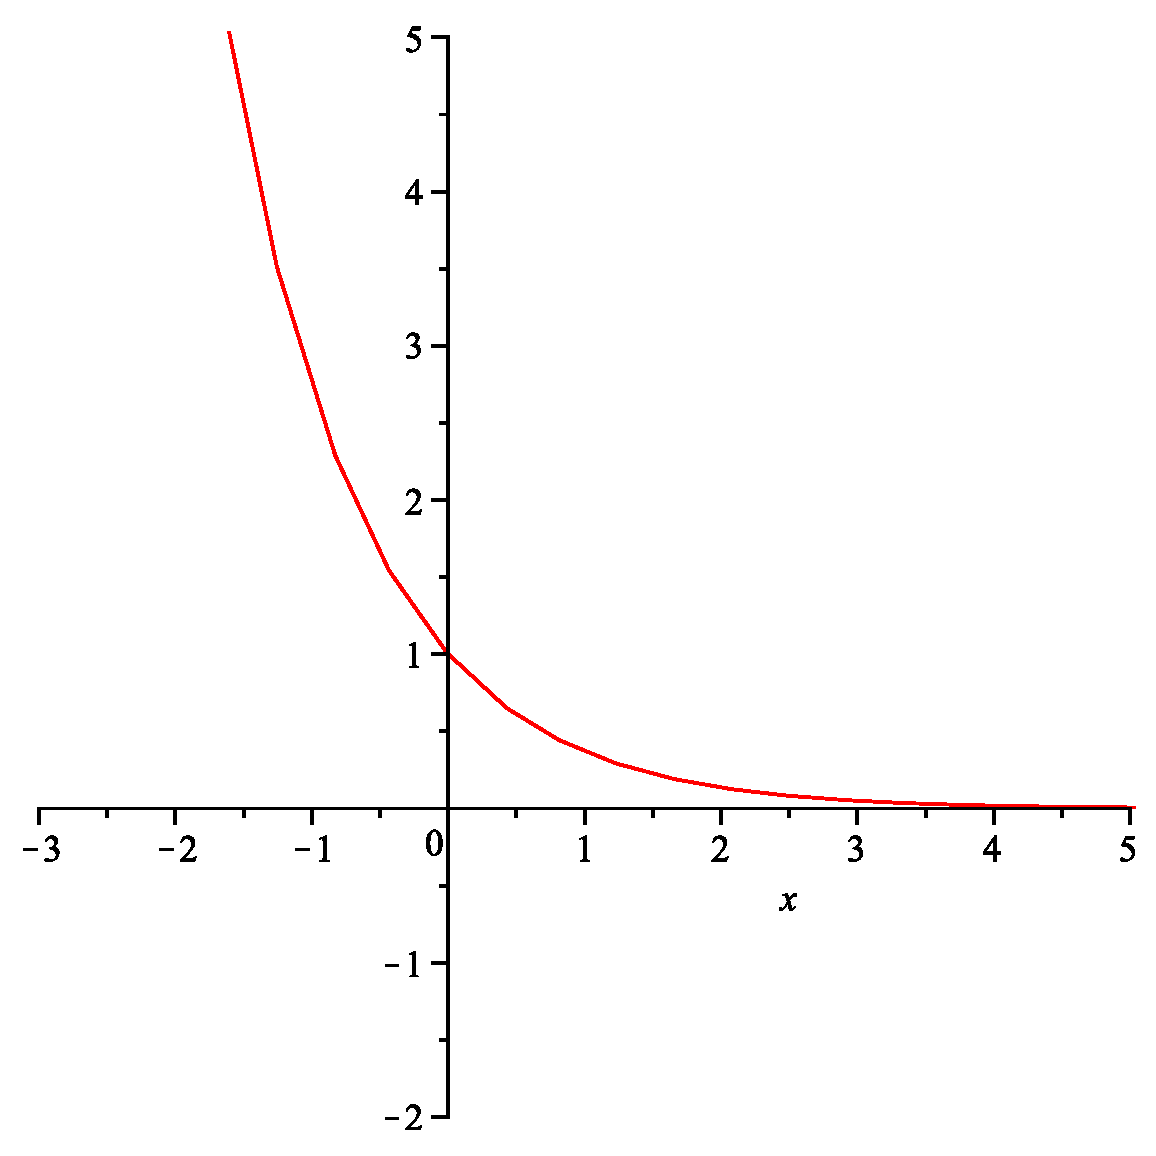
\includegraphics[scale=0.3]{imgs/fun01.pdf}}
  \label{fig:theFig}
  \caption{$f(x) = e^{-x}$}
\end{figure}

\begin{defn}[Punto di minimo locale]
 Un $\overline{x}$ si dice punto di minimo locale se
\begin{itemize}
 \item   $\overline{x} \in D$
 \item  $ \exists \varepsilon >0  \; | \; f(\overline{x}) \leq f(x) \; \forall x \in D \cap B(\overline{x}, \varepsilon)$
\end{itemize}
\end{defn}

\begin{figure}[h]
  \centerline{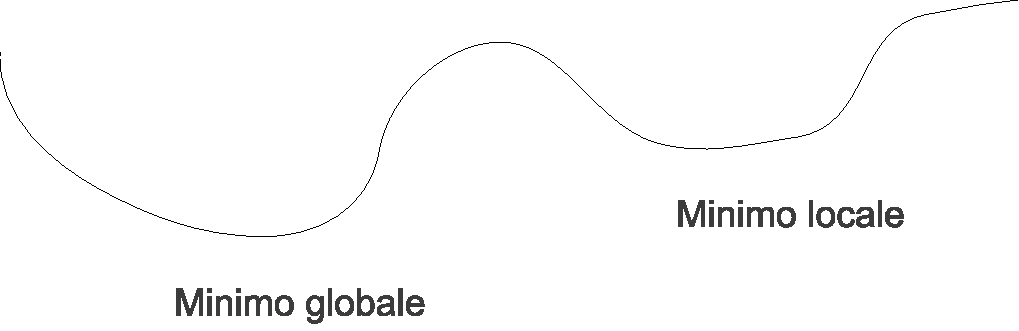
\includegraphics[scale=0.4]{imgs/img01.pdf}}
  \label{fig:theFi2}
  \caption{Minimo locale e globale}
\end{figure}

\begin{figure}[h]
  \centerline{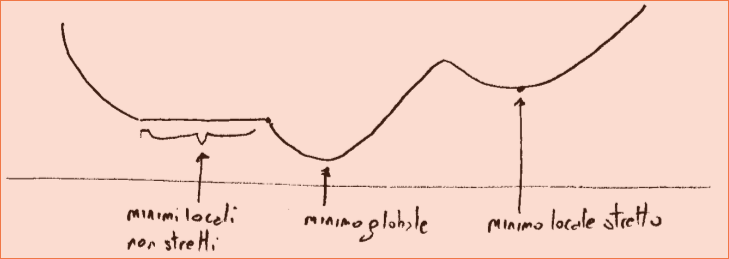
\includegraphics[scale=0.4]{imgs/img02.jpg}}
  \label{fig:theFi2}
  \caption{Minimo locale e globale}
\end{figure}

\begin{defn}[Punto di minimo locale stretto]
 Un $\overline{x}$ si dice punto di minimo locale stretto
di (P) se 
\begin{itemize}
 \item   $\overline{x} \in D$
 \item  $ \exists \varepsilon >0  \; | \; f(\overline{x}) < f(x) \quad  \forall x 
\in D \cap B(\overline{x}, \varepsilon), x \neq \overline{x}$
\end{itemize}
\end{defn}
Cioè il minimo è unico nell'intevallo selezionato.
\begin{defn}[Funzione convessa]
 Una $f: \mathbb{R}^n \rightarrow \mathbb{R}$ si dice \emph{convessa} se 
\begin{equation}
\label{richiamibigi:funzioneconvessa}
\forall x,y \in \mathbb{R}^{n}, \forall \lambda \in [0,1]
\qquad
f(\underbracket{\lambda x +(1-\lambda)y}_{\text{segmento } [x,y] \subseteq  \mathbb{R}^{n}}) \leq 
\underbracket{\lambda f(x) + (1-\lambda)f(y)}_{
\text{segmento } [f(x),f(y)] \subseteq \mathbb{R}
} 
\end{equation}
\end{defn}

\begin{defn}[Funzione concava]
 Una $f: \mathbb{R}^n \rightarrow \mathbb{R}$ si dice \emph{concava} 
 se la funzione $-f$ è convessa.
\end{defn}
\begin{figure}[!h]
  \centerline{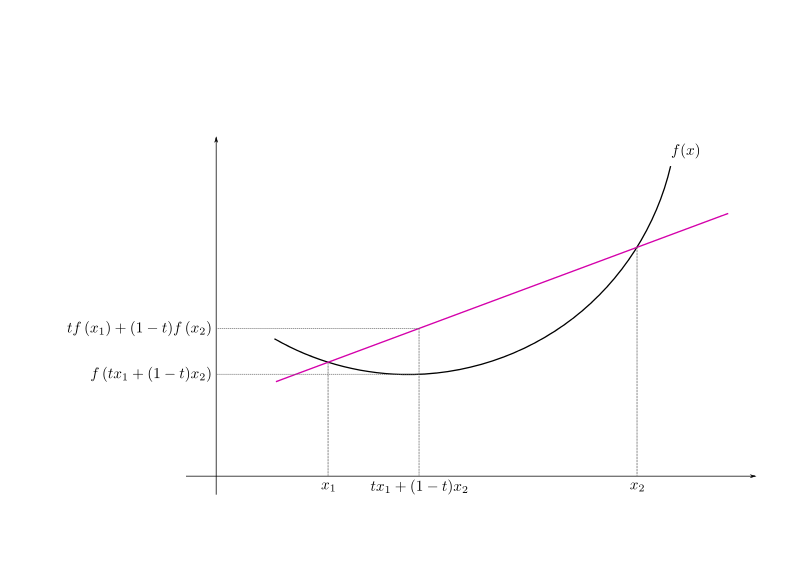
\includegraphics[scale=0.6]{imgs/img03.png}}
  \label{fig:theFi2}
  \caption{Funzione convessa}
\end{figure}

Si parla di \emph{funzioni strettamente convesse (concave)} se 
nella (\ref{richiamibigi:funzioneconvessa}) al posto
 di $\leq$ sostituiamo $<$ (simmetrico nel caso convesso).

 \begin{observation}
  $$ f \text{ \`e convessa } \; \Longleftrightarrow \;
f\left(\displaystyle \sum_{i=1}^{k} \lambda_i x_i \right) \leq 
\displaystyle \sum_{i=1}^{k} \lambda_i f(x_i)
\qquad
\forall x_1, \ldots, x_k \in \mathbb{R}^{n}, \forall \lambda_i \geq 0
\text{ con }  \displaystyle \sum_{i=1}^{k} \lambda_i = 1
$$
 \end{observation}

\begin{theo}[Locale $\equiv$ globale]
 Sia $f: \mathbb{R}^n \rightarrow \mathbb{R}$ convessa,
 $D \subseteq \mathbb{R}^n$ convesso. Allora ogni punto di minimo
 locale di (P) \`e anche un punto di minimo globale.
\end{theo}

Cioè nei problemi di ottimizzazione, se la regione ammissible è convessa,
e la funzione obiettivo \`e convessa, non c'\`e distinzione fra minimo locale e 
minimo globale.
\begin{thproof}

 Sia $\overline{x} \in D$ un minimo locale. Supponiamo, per assurdo,
che non sia un punto di minimo globale. Allora $\exists x$ tale 
che $f(x) < f(\overline{x})$. \\
Consideriamo il punto $x_{\lambda} = \lambda x + (1-\lambda)\hat{x}$
con $\lambda \in [0,1],  x_{\lambda} \in D$\\
Quanto vale la funzione in $x_{\lambda}$?
 $$f(x_{\lambda}) \underbracket{\leq}_{\text{convessit\`a}}  \lambda f(x) +
 (1-\lambda)f(\overline{x}) < \lambda f(\overline{x})
 + (1-\lambda) f(\overline{x})
 = f(\overline{x})$$
 $$ x_{\lambda} \xrightarrow{\lambda \rightarrow 0} \overline{x} \quad
  \forall \varepsilon  \exists  \overline{\lambda} \in [0,1] \quad 
 \text{ t.c. }  \quad x_{\overline{\lambda}} \in  B(\overline{x}, \varepsilon)$$
ed inoltre
$$ f(x_{\overline{\lambda}}) < f(\overline{x})$$
Quindi $\overline{x}$ non \`e un minimo locale (contraddizione)
\end{thproof}

\begin{defn}[Insieme convesso]
 $D \subseteq \mathbb{R}^{n}$ si dice \emph{convesso} se 
$\forall x,y \in D \; \forall \lambda \in [0,1]$:
$$ \underbracket{\lambda x + (1-\lambda)y}_{\text{segmento }  [x,y] \subseteq \mathbb{R}^{n}}\in D $$
\end{defn}

\begin{observation}
 Sono insiemi convessi
 \begin{itemize}
 \item $\mathbb{R}^{n}$
 \item $\emptyset$
 \end{itemize}
\end{observation}

\begin{figure}
  \centering
  \subfloat[Insieme convesso]{\label{fig:convexset}
    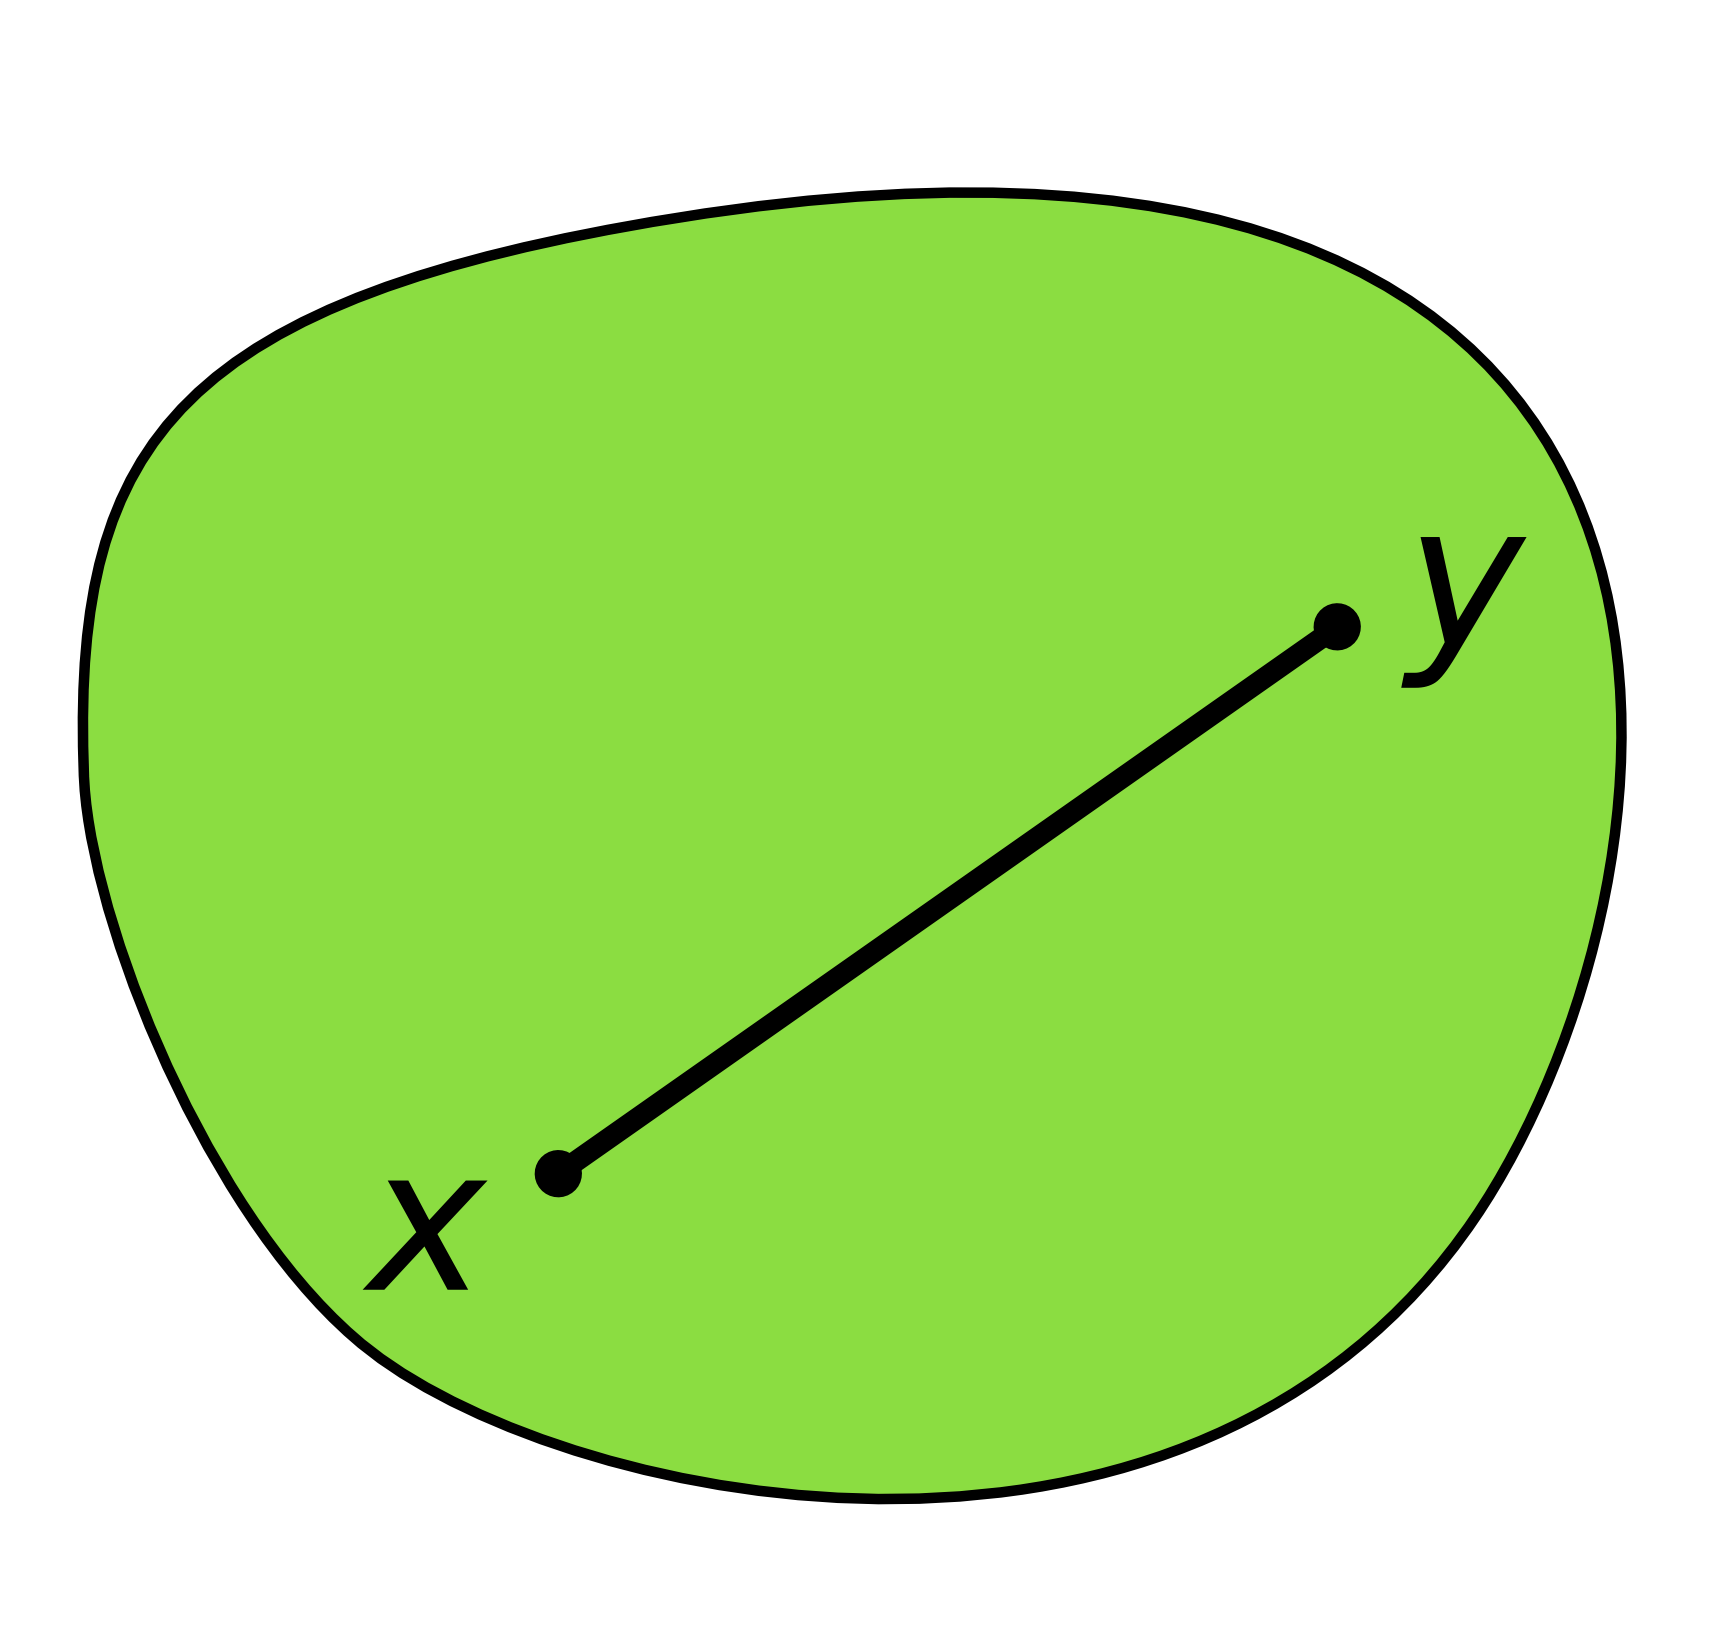
\includegraphics[width=0.25\textwidth]{imgs/img04.png}}                
  \subfloat[Insieme non convesso]{\label{fig:nonconvexset}
    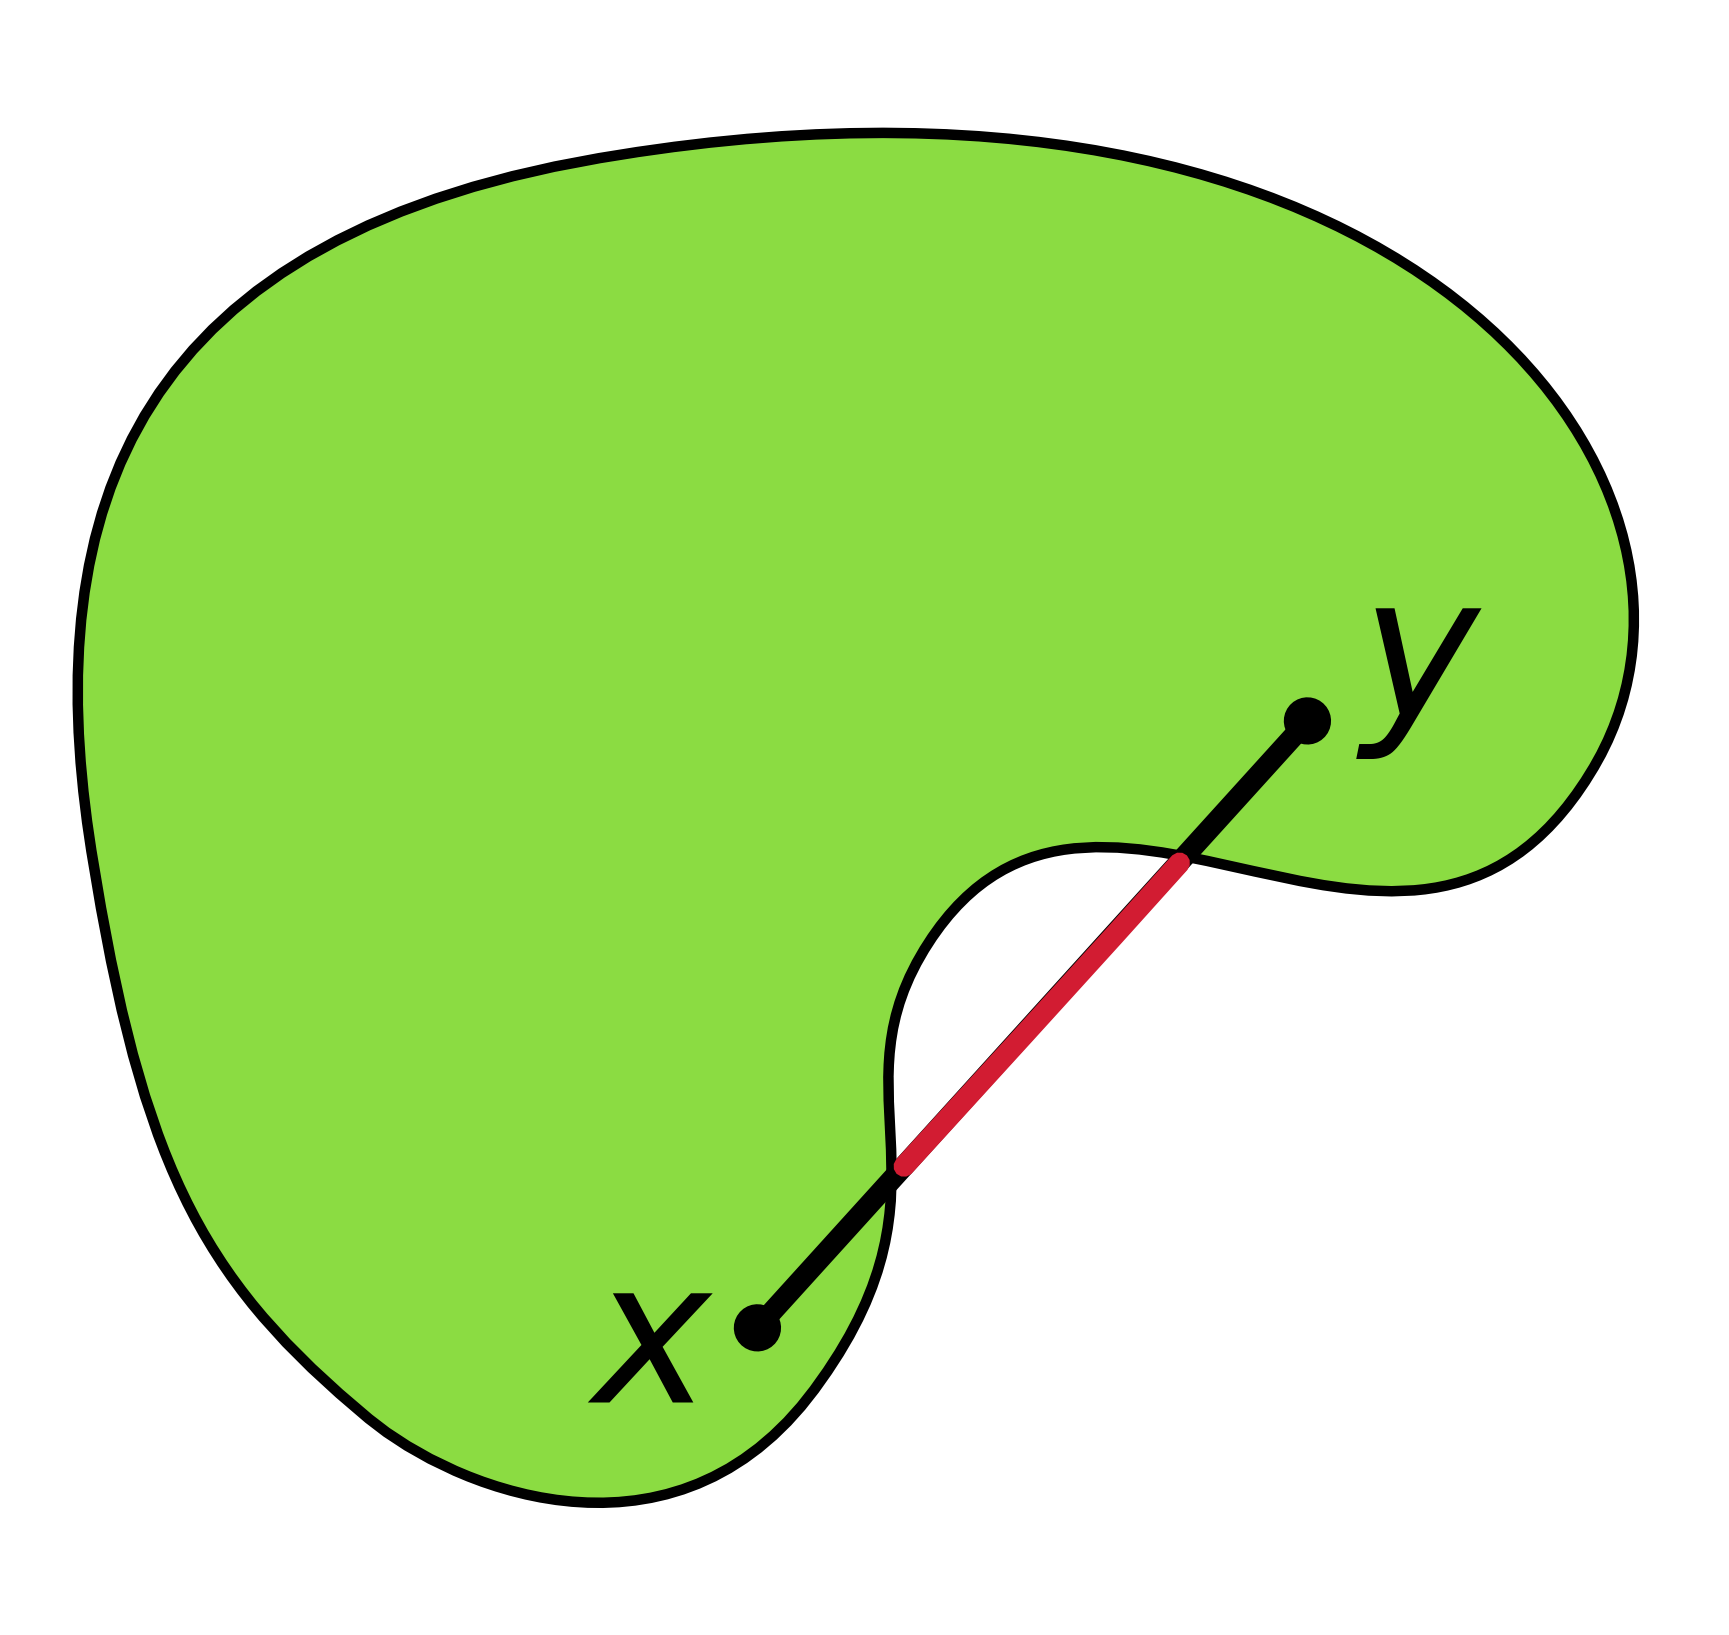
\includegraphics[width=0.25\textwidth]{imgs/img05.png}}
  \caption{Insiemi convessi e non convessi in $\mathbb{R}^2$}
  \label{fig:convexsets}
\end{figure}

\subsection{Risultati importanti su insiemi convessi
e funzione convesse}
\begin{theo}
 Sia $f: \mathbb{R}^n \rightarrow \mathbb{R}$ strettamente convessa,
$D \subseteq \mathbb{R}^n$ convesso. \\ Se (P) ammette un punto di
minimo, allora è l'unico punto di minimo.
\end{theo}

\begin{thproof}
 Sia $\overline{x} \in D$ minimo (globale $\equiv$ locale) di 
(P) e supponiamo esista $\hat{x} \in D$, $\hat{x} \neq \overline{x}$
 tale che $f(\hat{x}) = f(\overline{x})$. Sia $\lambda \in [0,1]
$ : $\lambda \hat{x} + (1-\lambda) \overline{x} \in D$
 (convessit\`a di D) e 
$$ f(\lambda \hat{x} + (1-\lambda)\overline{x}) < 
 \lambda f(\hat{x}) + (1-\lambda) f(\overline{x}) = 
 \lambda f(\overline{x}) + (1-\lambda)f(\overline{x}) =
  f(\overline{x})$$
  Quindi $\overline{x}$ non \`e un minimo 
 (globale $\equiv$ locale): contraddizione!
 \end{thproof}

\begin{notes}
 Ricordiamo che nel caso $D=\mathbb{R}^{n}$, $D$ è convesso, quindi abbiamo
automaticamente le proprietà sopra citate.
\end{notes}

\begin{notes}
Ricordiamo inoltre che i poliedri sono un insieme convesso, anche le
funzioni lineari, quindi nella programmazione lineare vale il il primo
teorema.
\end{notes}

\begin{property}
 $f$ convessa $\quad \Longrightarrow \quad f $ continua su
$\mathbb{R}^{n} $
\end{property}

\begin{property}
Sia $f: \mathbb{R}^{n} \rightarrow \mathbb{R}$.  Se $f$ è 
convessa, allora l'insieme di sottolivello
$$ C_{\alpha} = \{  x \in \mathbb{R}^{n} \; | \;  f(x) \leq \alpha \}$$
è convesso per ogni valore di $\alpha$
\end{property}

\begin{thproof}
Sia $C_\alpha \neq \emptyset$ e siano $x,y \in C_{\alpha}$. 
Allora $\forall \lambda \in [0,1]$ risulta
$$ f(\lambda x + (1-\lambda)y) \leq
 \lambda f(x) + (1-\lambda) f(y) \leq \lambda \alpha
 + (1-\lambda) \alpha = \alpha$$
da cui $\lambda x + (1-\lambda)y \in C_{\alpha}$
\end{thproof}

\begin{observation} Per vedere che quest'ultima proprietà vale solo in un
senso, basta prendere la funzione $ x^{3}$, che non è convessa. I
sottolovelli sono tutti insiemi convessi.
 $$ C_{\alpha} = (-\infty, \sqrt[3]{\alpha})$$
\end{observation}

\begin{property}
  Siano  $f_i: \mathbb{R}^{n} \rightarrow \mathbb{R} $ una famiglia di
funzione convesse,  $k \in \mathbb{N}$  finito. Allora
  \begin{enumerate}
  \item $ \displaystyle \sum_{i=1}^{k} f_i $ è convessa
  \item $ \displaystyle \sup_{i \in I} f_i $ è convessa
  \end{enumerate}
\end{property}

\begin{thproof}
  \begin{enumerate}
  \item Ovvio: basta applicare la definizione ad ogni $f_i$ e
 sommare membro a membro
 \item
Nel caso $I$ sia finito allora
 $$(\sup f_i) = (\lambda x + (1-\lambda) y= 
 f_k (\lambda x + (1-\lambda)y) \leq f_k(x) + (1-\lambda) f_k(y)
 \leq \lambda (\sup f_i)(x) + (1-\lambda) (\sup f_i) (y)$$
per un $k$ opportuno
  \end{enumerate}
\end{thproof}

\begin{theo}
\label{richiamibigi:theo01}
 Sia $f$ differenziabile (su $\mathbb{R}^{n}$)
 $$  f \text{  è convessa } \Longleftrightarrow f(y) \geq  f(x) + \underbracket{ \nabla f(x)^{T} (y-x)}_{\text{piano tangente}} \quad \forall x, y \in \mathbb{R}^{n}$$
\end{theo}
 Informalmente: il grafico di $f$ sta sopra il piano tangente.
 Ricordiamo che $||x||$ è convessa ma non è differenziabile
\begin{thproof} $\Longrightarrow$ \\ $x,y \in \mathbb{R}^{n}, \lambda
\in [0,1]$ \\
$$
\begin{array}{ll}
\lambda f(y) + (1- \lambda) f(x)  \geq f(\lambda y + (1-\lambda)x)  & \Rightarrow \\
   \lambda f(y) -  \lambda f(x)  \geq f(\lambda y + (1-\lambda)x) -f(x) & \Rightarrow \\
   f(y) -  f(x)  \geq \dfrac{f(\lambda x + (1-\lambda)y) -f(x)}{\lambda}  \xrightarrow{\lambda \to 0} 
 \nabla f(x)^{T} (y-x) &
 %  f(y) -  f(x)  \geq \dfrac{f(\lambda x + (1-\lambda)y) -f(x)}{\lambda} 
 % % y + (1-\lambda) x = x + \lambda(y-x)  
 % %  f(y) -  f(x)  \geq \frac{f(x +  \lambda(y-x))}{\lambda} \rightarrow_{\lambda \rightarrow 0} 
 % % \nabla f(x)^{T} (y-x)
\end{array} 
$$
  \\ \\
 $\Longleftarrow$ \\
  $x,y \in \mathbb{R}^{n}, \lambda \in [0,1]$ \\
  \begin{equation}
    \label{eq01:001}    
f(x) - f(\lambda y + (1-\lambda)x) \geq 
  \nabla f(\lambda y  + (1 - \lambda)x)^{T}[\lambda(x-y)]
  \end{equation}
  \begin{equation}
    \label{eq01:002}    
f(y) - f(\lambda y + (1-\lambda)x ) \geq 
  \nabla f(\lambda y  + (1 - \lambda)x)^{T}[(\lambda -1)(x-y)]
  \end{equation}

% $$1) \quad f(x) - f(\lambda y) + (1-\lambda)x) \geq \lambda \nabla f(\lambda  + (1-\lambda)x)^{T} (x-y)$$

% $y -\lambda y - (1-\lambda)x \rightarrow (1-\lambda) (y-x)$
% $$2) \quad f(x) - f(\lambda y) + (1-\lambda)x) \geq (\lambda-1) \nabla f(\lambda y  + (1-\lambda)x)^{T} (x-y)$$
% Moltiplichiamo 1) per $1-\lambda$.
% $$1) (1-\lambda) [ f(x) - f(\lambda y) + (1-\lambda)x)] \geq (1-\lambda)\lambda   \nabla f(\lambda  + (1-\lambda)x)^{T} (x-y)$$
% Moltiplichiamo 2) per $\lambda$.
% $$  \lambda[f(x) - f(\lambda y) + (1-\lambda)x)] \geq (\lambda-1)\lambda \nabla f(\lambda y  + (1-\lambda)x)^{T} (x-y)$$
% Allora la somma a membro a membro di 1) e 2)
% $$(1-\lambda) f(x) + \lambda f(y) \geq f(\lambda y + (1-\lambda) x)$
%$
$$(1-\lambda) (\ref{eq01:001}) 
+ \lambda (\ref{eq01:002})
\quad \Rightarrow \quad 
(1-\lambda) f(x) + \lambda f(y) \geq
(1-\lambda)f(\lambda y + (1-\lambda)x) + \lambda f(\lambda y +
(1-\lambda)x) = f(\lambda y + (1-\lambda)x)
$$
che è la disuguaglianza di convessità
\end{thproof}
\begin{todo}
Ho lasciato commentato la dimostrazione presa a lezione
di quest'ultimo teorema perch\`e pi\`u verbosa. Vedere se ha senso
 fare un'integrazione con quella attuale.
\end{todo}

\begin{theo}
\label{richiamibigi:theo02} 
Sia $f$ differenziabile 2 volte (su $\mathbb{R}^{n}$). Allora
 $$ f \text { è convessa } \Longleftrightarrow \nabla^{2} f(x) \text{ è semidefinita positiva} \quad \forall x \in \mathbb{R}^{n},
\text{ovvero } y^{T}\nabla^{2}f(x)y \geq 0
$$
\end{theo}

\begin{thproof}
\begin{itemize}
\item[$ \Longleftarrow$]
 $x,y \in \mathbb{R}^{n}, \quad \lambda  \in \mathbb{R}$

\begin{equation}
  \label{richiamibigieq:003}
f(x+ \lambda y) - \underbracket{f(x)}_{} -\nabla f(x)^{T}y \geq 0
\qquad (\text{Teorema } (\ref{richiamibigi:theo01})\;)   
\end{equation}
Sfruttando Taylor di secondo ordine
\begin{equation}
  \label{richiamibigieq:004}
  f(x) = \frac{1}{2} \lambda^{2} y^{T} \nabla^2 f(x) y + r(\lambda y)
\end{equation}
\begin{enumerate}
\item dividendo (\ref{richiamibigieq:004}) per $\lambda^{2}$
 \item utilizzando la relazione
$||\lambda y||_{2}^{2} = \lambda^{2} ||y||_{2}^{2} = \lambda^{2}$
 \item mettendo insieme (\ref{richiamibigieq:003})  e (\ref{richiamibigieq:004})
\item $\dfrac{r(h)}{||h||_{2}} \xrightarrow{|| h||_{2} \ \to 0} 0$
\end{enumerate}
otteniamo
$$ \frac{1}{2} y^{T} \nabla^{2}f(x) y   + \frac{r(\lambda y)}{\lambda^2}  \geq  0
\quad
\xrightarrow{\lambda \to 0} 
\quad
 \frac{1}{2} y^{T} \nabla^{2}f(x) y   \geq  0
\quad
\Longrightarrow \quad
y^{T} \nabla^{2} f(x) y \geq 0 
$$
che era quello che volevamo dimostrare.

\item[$\Longrightarrow$]
 Siano $x,y \in \mathbb{R}^{n}$. 
$$f(y) - f(x) - \nabla f(x)^{T}(y-x)
\underbracket{ =}_{\text{Taylor}} \frac{1}{2} (y-x)^{T} \nabla^{2} f(x + t(y-x))(y-x) \underbracket{\geq}_{\text{ipotesi}} 0$$
 Questo vale per un $t \in (0,1)$ opportuno.
Dal teorema (\ref{richiamibigi:theo01}) otteniamo immediatamente
che $f$ \`e convessa, che era la nostra tesi.
\end{itemize}
\end{thproof}

\begin{observation}[Casi particolari dei precedenti teoremi/proposizioni]
$$f \text{ concava} 
\left\{
\begin{array}{l}
\text{ Teorema } (\ref{richiamibigi:theo01}) \text{ con }
  f(y) \leq f(x) + \nabla f(x)^{T}(y-x) \\
\text{ Teorema } (\ref{richiamibigi:theo02}) \text{ con }
  \nabla^{2}f(x) \text{ semidefinita negativa } (y^{T} \nabla f(x)y \leq 0)
\end{array}
\right.
$$
$$
f \text{ strettamente convessa} 
\left\{
\begin{array}{ll}
\text{ Teorema }   (\ref{richiamibigi:theo01}) & \text{ con }
  f(y) > f(x) + \nabla f(x)^{T}(y-x) \quad (y\neq x) \\
\text{ Teorema }   (\ref{richiamibigi:theo02}) & 
   \text{ vale la parte necessaria con }
  \nabla^{2}f(x) \text{ semidefinita positiva}  \\
 & [\text{e non definita positiva}]: \nabla^{2}f(x) \Rightarrow f \text{ strettamente convesso} 
\end{array}
\right.
$$
Ad esempio: $n=1$, $f(x)=x^{4}$ \`e strettamente convessa ma
$\nabla^{2}f(0) = 0$ [$\nabla^{2}f(x)=12x^2$]
\end{observation}

\begin{defn}[Epigrafico]
$$ epi(f) = \{ (x,t) \; | \; x \in \mathbb{R}^{n}, t \geq f(x) \}
\subseteq \mathbb{R}^{n+1}
$$
\end{defn}
%Un modo informale per descrivere l'epigrafico \`e
%l'insieme di punti che stanno al di sopra o sul grafico di una

\begin{property}
Sia $f: \mathbb{R}^{n} \rightarrow \mathbb{R}$ 
$$f  \text{ è convessa } \quad   \Longleftrightarrow  
 \quad epi(f)
 \text { è convesso}$$
\end{property}

\begin{thproof}
\begin{itemize}
\item[$\Longrightarrow$]
 Siano $(x,t), (y,\tau) \in epi(f), \lambda \in [0,1]$:
$$
\lambda t + (1-\lambda) \tau \geq \lambda f(x) + 
(1-\lambda) f(y) \underbracket{\geq}_{\text{convessit\`a}}
f(\lambda x + (1-\lambda)y)
$$
da cui
$$ (\lambda x + (1-\lambda) y, 
\lambda t + (1-\lambda) \tau) \in epi(f)
$$
\item[$\Longleftarrow$]
Siano $x,y \in \mathbb{R}^{n}, \lambda \in [0,1]:
 (x,f(x)) ,(y,f(y)) \in epi(f)$

$$ epi(f) \text{ convesso} \quad
\Longrightarrow \quad
(\lambda x + (1-\lambda) y, \lambda f(x) + (1-\lambda) f(y)
 \in epi(f) 
$$
ovvero
$$ \lambda f(x) + (1-\lambda)f(y) \geq f(\lambda x + (1-\lambda)y)$$
\end{itemize}

\end{thproof}




\begin{notes}
 Tali teoremi possono essere riscritti per le funzioni convesse
\end{notes}

\begin{todo}
 Scrivere bene proprietà per funzioni convesse e strettamente convesse
\end{todo}
$$f(x) = x^4 \quad \nabla f(x) = 4x^{3} \quad \nabla^{2} f(x) = 12 x^{2} $$ 
La matrice hessiana non è definita positiva. \\ \\

\begin{proposition}
 Siano $f$ convessa, $D$ convesso. Allora l'insieme dei punti di minimo
 di $(P)$ è convesso.
\end{proposition}

Infatti  $\overline{x}, \hat{x} \in D$ minimi $f(\overline{x}) = f(\hat{x})$.
  $$ f(x_{\lambda}) \leq  \lambda f(\overline{x}) + 
  (1-\lambda) f(\hat{x})  = f(\hat{x}) = f(\overline{x})
  \quad \rightarrow \quad  f(x_{\lambda}) = f(\overline{x})$$
  Cioè $x_{\lambda}$ è minimo.

\paragraph{Funzioni quadratiche e convessit\`a}
 $Q \in \mathbb{R}^{n \times n} , b \in \mathbb{R}^{n},
 Q \text{ simmetrica }, c \in \mathbb{R}$

$$ f(x) = \dfrac{1}{2} x^{T}Qx + b^{T}x + c
\quad \Longrightarrow \quad f \text{ differenziabile 2 volte:}
\nabla^{2}f(x) \equiv Q \quad \forall x
$$
Dal teorema (\ref{richiamibigi:theo02}) seguono:
\begin{property}
$f$ \`e convessa $\; \Longleftrightarrow \; Q$ \`e semidefinita positiva,
ossia gli autovalori di $Q$ sono tutti $\geq 0$
\end{property}

\begin{property}\label{prop:quadratica-defpos-convessa}
$Q$ definita positiva $\; \Longrightarrow \; f$ \`e strettamente convessa
\end{property}



\section{Ottimizzazione non vincolata}
%% 19 Novembre
$D = \mathbb{R}^{n}$ ottimizzazione \emph{non vincolata}: $(P) \quad \min\{f(\mathbf{x}): \mathbf{x} \in \mathbb{R}^{n}\}$
\subsection{Condizioni di ottimalit\`a}
\begin{theo}[Condizioni necessarie del primo e del secondo ordine] Sia
$\mathbf{\overline{x}} \in \mathbb{R}^{n}$ un punto di minimo locale di (P).
\begin{enumerate}
 \item Se $f$ \`e differenziabile in $\mathbf{\overline{x}}$, allora
$\nabla f(\mathbf{\overline{x}}) = \mathbf{0}$
 \item Se $f$ \`e differenziabile 2 volte in $\mathbf{\overline{x}}$,
allora $\nabla^{2}f(\mathbf{\overline{x}})$ (la matrice Hessiana) \`e
semidefinita positiva.
\end{enumerate}
\end{theo}

\begin{thproof} Sia $ \varepsilon > 0$ tale che $f(\mathbf{\overline{x}})
= \min \{ f(\mathbf{x}) = \mathbf{x} \in B(\mathbf{\overline{x}},
\varepsilon)\}$, e siano $\mathbf{d} \in \mathbb{R}^{n}$ con
$||\mathbf{d}||_{2}=1$ una direzione e $ t \leq \varepsilon$:
 \begin{enumerate}
  \item Per ipotesi $\mathbf{\overline{x}}$ è punto di minimo locale,
quindi
 $$ \exists \varepsilon > 0.  \quad f(\mathbf{\overline{x}}) 
\leq f(\mathbf{x}) \quad \forall \mathbf{x} \in 
B(\mathbf{\mathbf{\overline{x}}}, \varepsilon)$$

sappiamo che vale la seguente relazione (Taylor):
$$ 0 \leq f(\mathbf{\overline{x}} + t\mathbf{d}) - f(\mathbf{\overline{x}}) = 
t \nabla f(\mathbf{\overline{x}})^{T}\mathbf{d} + r(t \mathbf{d}) $$

da cui
$$ 0 \leq \nabla f(\overline{x})^{T}\mathbf{d} + \dfrac{r(t\mathbf{d})}{t} \xrightarrow{t \to 0}
\nabla f(\overline{x})^{T}\mathbf{d}$$ ovvero $\nabla
f(\overline{x})^{T}\mathbf{d} \geq 0$ Analogamente, utilizzando la
direzione $(-\mathbf{d})$ si ottiene $\nabla
f(\overline{x})^{T}\mathbf{d} \leq 0$.  Quindi
$$\nabla f(\mathbf{\overline{x}})^{T}\mathbf{d} =0 \quad \forall \mathbf{d} \in \mathbb{R}^{n}$$
(con $||\mathbf{d}||_{2}=1$), da cui $\nabla
f(\mathbf{\overline{x}})=0$ (considerare $d = \nabla
f(\mathbf{\overline{x}})$)

%% OLD VERSION
% $$ 0 \leq \frac{f(\overline{x} +td) = f(\overline{x})}{t} \underbracket{=}_{\text{Taylor}}
% t \nabla f(\overline{x})^{T}d + \frac{r(td)}{t} \rightarrow_{t\rightarrow 0} 
% \nabla f(\overline{x})^{T} d$$ Quindi
% $$ \nabla f(\overline{x})^{T} d \geq 0$$
% $d$ è una direzione qualsiasi, si potrebbe ripetere lo stesso
%ragionamento per $-d$
%  $$ \nabla f(\overline{x})^{T}  d \leq 0$$
% Unendo le due abbiamo
% $$ \nabla f(\overline{x})^{T} d = 0$$
% L'unico vettore che soddifa ci\`o è il vettore nullo ossia % $\nabla
%f(\overline{x}) = 0$

\item La prima parte della dimostrazione è analoga. \\ Riscriviamo lo
sviluppo di Taylor, questa volta del secondo ordine. (La funzione è
differenziabile 2 volte)
 $$ 0 \leq f(\overline{\mathbf{x}} + td) - f(\overline{\mathbf{x}}) =
 \underbracket{t \nabla f(\overline{\mathbf{x}})^{T} \mathbf{d}}_{(*)}
+ \frac{1}{2} t^{2} \mathbf{d}^{T} \nabla^{2} f(\overline{\mathbf{x}})
\mathbf{d} + r(t\mathbf{d}) = \frac{1}{2} t^{2} \mathbf{d}^{T}
\nabla^{2} f(\overline{\mathbf{x}}) \mathbf{d} + r(t\mathbf{d})
$$
Dividendo per $t^2$ otteniamo:
 $$ 0 \leq \frac{f(\overline{\mathbf{x}} + t\mathbf{d})}{t^2} = 
\frac{1}{2} \underbracket{\mathbf{d}^{T}\nabla^{2} f(\overline{\mathbf{x}})} \mathbf{d}
 + \frac{r(t\mathbf{d})}{t^2} 
$$
Facendo tendere $t$ a 0 otteniamo
$$
{t \rightarrow 0 \quad \Rightarrow \quad 0 \leq \frac{1}{2}
\mathbf{d}^{T} \nabla^{2}f(\overline{\mathbf{x}})\mathbf{d}} +
\cancel{\frac{r(t\mathbf{d})}{t^2}}
$$
Concludiamo quindi che
 $$ \mathbf{d}^{T} \nabla^{2} f(\overline{\mathbf{x}})\mathbf{d}
 \geq 0 \; \forall \mathbf{d}  \in \mathbb{R}^{n}, ||\mathbf{d}||_{2} = 1
$$
L'ultima è la definzione di matrice semidefinita positiva.
 \end{enumerate}
\begin{notes} 
\begin{itemize}
\item[(*)] \text{Questa quantità sparisce per il punto 1}
\end{itemize}
\end{notes}


\end{thproof}
\begin{theo}[Caso Convesso] Sia $f$ una funzione convessa e
differenziabile su $\mathbb{R}^{n}$. Allora
$$ x \in \mathbb{R}^{n}
\text{ \`e un di minimo (locale e globale) di (P)} \quad \Longleftrightarrow \quad
\nabla f(\overline{x}) = 0
$$
\end{theo}
\begin{thproof} $\Rightarrow$: \ dimostrato dal teorema precedente \\
$\Leftarrow$:
 $$ f \text{ convessa }  \quad \Longrightarrow \quad  f(y) \geq f(\overline{x}) +
 \underbrace{\nabla f(\overline{x})^{T}(y-x)}_{\text{questo pezzo sparisce}} \quad
 \forall y \in \mathbb{R}^{n} 
$$
$$ \nabla f(\overline{x}) = 0  
\quad \Longrightarrow \quad f(y) \geq f(\overline{x}) \quad \forall y
\in \mathbb{R}^{n} \quad \Longrightarrow \quad \overline{x}
 \text{ \`e un punto di minimo }
 $$
\end{thproof}

%%% FROM HERE

\begin{example}
$$ f(x_1, x_2) =  (x_2, -x_1^{2}) (x_2 - 4x_{1}^2) [ = x_2^{2} - 5x_1^{2}x_2 + 4x_{1}^{4}]$$
 $$ \nabla f(\mathbf{x}) = 
\begin{pmatrix}
-10 x_1 x_2 + 16 x_1^3\\
2 x_2 - 5 x_1^2
\end{pmatrix}
$$
$$
\nabla f(\mathbf{x}) = 0
\quad 
\Longleftrightarrow
\quad
\left\{
\begin{array}{ll}
 2x_{2} = 5x_1^{2} \\
 16x_{1}^{3} = 10x_1 x_2 
\end{array}
\right.
\quad 
\Longleftrightarrow
\quad
x_1 = x_2 =0
$$
Il gradiente si annulla se
$\mathbf{x}$ è il vettore nullo. \\

Vediamo la matrice Hessiana:
$$ \nabla^{2}f(\mathbf{x}) =
\begin{pmatrix}
 -10 x_2 + 48x_1^{2} & -10x_1 \\
  -10x_1 & 2
\end{pmatrix}
$$
Calcoliamo in $(0,0)$.
$$ \nabla^{2} f((0,0)) =
\begin{pmatrix}
 0 & 0 \\
 0 & 2
\end{pmatrix}
$$
Semidefinita positiva, ma non è definita positiva (in quanto ha uno zero  nella diagonale) \\
Calcoliamo in $(0,1)$.
$$ \nabla^{2} f((0,1)) =
\begin{pmatrix}
 -10 & 0 \\
 0 & 2
\end{pmatrix}
$$
Questa non è definita positiva ( negativa) quindi $f$ non è convessa.
$ f(0,0) = 0$

$$ P = \{x_2 = 2x_1^2 \}
\quad
 f(x_1, 2x_1^2) = -2x_1^{4} < 0 \quad \text{ se }  x_1 \neq 0$$
$f$ \`e negativa su $P|\{\overline{x}\} :
\quad x_k = (\frac{1}{k}, \frac{2}{k^2})
\quad x_k \rightarrow \overline{x}
\text{ e }
f(x_k) = \frac{-2}{k^4} <0$ \\
Possiamo concludere che $\overline{\mathbf{x}} = (0,0)$ non è un minimo locale.
\end{example}


\begin{defn}[Punto Stazionario]
 $\overline{x} \in \mathbb{R}^{n}$ si dice punto stazionario per $f$ se $\nabla f(\overline{x}) = 0$
\end{defn}


\begin{theo}[Condizione sufficiente]
\label{theo:punto-stazionario-minimo-locale}
Sia $f$ differenziabile 2 volte in $\overline{x} \in \mathbb{R}^{n}$ e valga
$\nabla f(\overline{x})=0$. (Punto stazionario) \\
 Se $\nabla^{2}f(\overline{x})$ è definita positiva,
allora $\overline{x}$ è un punto di minimo locale \emph{stretto} di (P), ed inoltre
esistono $\gamma > 0$ e $\delta >0$ tali che:
$$ f(x) \geq f(\overline{x}) + \gamma || x- \overline{x} ||^{2}_{2} \quad \forall x \in B(\overline{x}, \delta)$$
\end{theo}
\begin{thproof}
\begin{notes}
La dimostrazione data a lezione \`e lievemente diversa
, ma solo per la notazione: lascio commentata nel sorgente
Tex
\end{notes}
Sia $x \in \mathbb{R}^{n}$

$$
\begin{array}{l}
 f(x) - f(\overline{x}) = \\
 \nabla
f(\overline{x})^{T}(x - \overline{x}) +
\dfrac{1}{2}(x-\overline{x})^{T}
\nabla^{2}f(\overline{x})(x - \overline{x})
+ r(x - \overline{x}) \underbracket{ = }_{*)}
 \\
\dfrac{1}{2}(x-\overline{x})^{T}
\nabla^{2}f(\overline{x})(x - \overline{x})
+ r(x - \overline{x})
\end{array}
$$
Sia $\lambda_{min}>0$ il pi\`u piccolo autovalore di
$\nabla^{2}f(\overline{x}) 
(\Rightarrow y^{T} \nabla^{2}f(\overline{x})y \geq
\lambda_{min} ||y||_{2}^{2} \; \forall y \in \mathbb{R}^{n}
)$ 
$$f(x) - f(\overline{x}) \geq \dfrac{\lambda_{min}}{2}
|| x - \overline{x} ||_{2}^{2} + r(x - \overline{x}) 
 $$
$$
\dfrac{f(x)-f(\overline{x})}{||x - \overline{x}||_{2}^{2}}
\geq \dfrac{\lambda_{min}}{2}
 + \dfrac{r(x - \overline{x})}{|| x - \overline{x} ||_{2}^{2}}
\xrightarrow{x \to \overline{x}} \dfrac{\lambda_{min}}{2}
 $$
Sia $0 < \varepsilon < \dfrac{\lambda_{min}}{2}$ :
per la definizione di limite esiste $\gamma > 0$ tale che
$$
\dfrac{f(x) - f(\overline{x})}{||x - \overline{x}||_{2}^{2}}
\geq (\dfrac{\lambda_{min}}{2} - \varepsilon) = \gamma
\quad \forall x \in B(\overline{x},\delta)
$$
da cui
$$ f(x) \geq f(\overline{x}) + \gamma || x - \overline{x}||_{2}^{2} \quad \forall x \in B(\overline{x},\delta)$$
\begin{itemize}
\item[*)] $\nabla f(\overline{x})=0$
\end{itemize}

% \\
%  $d \in \mathbb{R}^{n}, ||d||_{2} = 1 $ \\
%  $$ f(\overline{x} + td) - f(\overline{x}) = \underbracket{t \nabla f(\overline{x}^{T}d}_{0 \text{ per ipotesi} } + 
%  \frac{1}{2}t^{2}d^{T}\nabla^{2}f(\overline{x})d + r(td)$$
% $$ \frac{f(\overline{x} + td) - f(\overline{x}) }{t^{2}} = \frac{1}{2} d^{T} \nabla^{2}f(\overline{x})d + \frac{r(td)}{t^2}$$
% Usiamo una proprietà delle matrici semidefinite positive.
% $$ d^{T}A d \geq \lambda_{\min}||d||_{2}^{2}$$
% più piccolo autovalore di A.
% $$ \frac{f(\overline{x} + td) - f(\overline{x}) }{t^{2}} = \frac{1}{2} d^{T} \nabla^{2}f(\overline{x})d + \frac{r(td)}{t^2}
% \geq_{\lambda_{\min} > 0} \frac{1}{2} \lambda_{\min} +  \frac{r(td)}{t^2} \rightarrow_{t \rightarrow 0} \frac{1}{2} \lambda_{\min}
% $$
% Prendiamo $\varepsilon < \frac{\lambda_{\min}}{2}$ \\
% Per definizione di limite 
% $$\exists \; \delta \; \text {t.c.} \; \frac{ f(\overline{x}+td) - f(\overline{x})}{t^2} \geq \frac{\lambda_{\min}}{2} - \varepsilon \quad \forall t \in [0, \delta)$$

% $$x \in B(\overline{x}, \delta) \quad  x = \overline{x}+td \quad 0 < t < \delta, d \in \mathbb{R}^{n}, ||d||_{2} = 1 \text{ opportuni}$$
% Ricordiamo che:
% $$ d = \frac{ x - \overline{x}}{||x - \overline{x}||_{2}} \quad t = || x = \overline{x}||_{2} < \delta $$
% Ma allora abbiamo finito, infatti:
% $$ \frac{f(x) - f(\overline{x})}{||x - \overline{x}||_{2}^{2}} \geq \gamma$$
\end{thproof}

\begin{observation}[Risultati per i punti di massimo]
 $$\max \{ f(x): x \in \mathbb{R}^{n}\} = -min \{  -f(x): x \in \mathbb{R}^{n} \}$$
Quindi per le condizioni di massimo non dobbiamo dimostrare nulla.\\
Cambia il punto (2) (semidefinita positiva) che diventa semidefinite negativa.
Per i punti di massimo locale la matrice deve essere la matrice definita negativa, otterremo
un punto di massimo locale stretto. \\ \\
\end{observation}

\begin{observation}
Ad eccezione di quelle costanti, le funzioni convesse
 (differenziabili) non ammettono punti di massimo locale/globale
su $\mathbb{R}^{n}$:
$$ \overline{x} \text{ \`e massimo di } f
\quad \Longrightarrow \quad
\nabla f(\overline{x}) = 0
$$
ma
$$
f \text{ convessa } \; \wedge \;
\nabla f(\overline{x}) = 0 
\quad \Longrightarrow \quad 
\overline{x} \text{ minimo di f} $$
Abbiamo un punto di massimo e di minimo,quindi
$f$ \`e costante.
\end{observation}

\begin{exercise}
$$\nabla f \neq 0 \quad \nabla f(x) \neq 0 \quad y(t) = t \nabla f(x) + x$$
Dimostrare che $f(y(t)) \rightarrow_{t\rightarrow +\infty} + \infty$  \\
Suggerimento : usare
$$ f(y) \geq f(x) + \nabla f(x)^{T} (y-x)$$
\end{exercise}

\begin{observation}[Funzioni Quadratiche]
La funzioni quadratiche non convesse
 $$f(x) = \frac{1}{2} x^{T} Qx + b^Tx + c \qquad Q \in \mathbb{R}^{n \times n} \text {simmetrica }, b \in \mathbb{R}^{n}, c \in \mathbb{R} $$
non ammettono minimo locale in quanto
$\nabla^{2}f(x) \equiv Q$ non \`e definita positiva
% \begin{itemize}
%  \item $\nabla^{2} f(x) = Q$: non ammettono punti di minimo locale.
%  \item $\nabla f(x) = Qx +b$.
% \end{itemize}
\end{observation}
\paragraph{Legami con l'analisi numerica}

\subparagraph{Funzioni quadratiche}
 Chiedere ad una funzione quadratica che
    $$ \nabla f(x^{*})=0 \quad \Longleftrightarrow \quad Q x^{*} = -b $$
   è la stessa cosa di risolvere il seguente sistema lineare:
 $$Qx = -b$$
Questo è un primo legame con l`analisi numerica. \\

\subparagraph{Caso generale}
$$ \nabla f : \mathbb{R}^{n} \rightarrow \mathbb{R}^{n}$$
In generale il gradiente è una funzione non lineare. Trovare i punti stazionari è sostanzialmente risolvere un sistema
di equazioni non lineari.
$$
\left\{
\begin{array}{l}
\frac{\partial f}{\partial x_1} (x) = 0 \\
 \frac{\partial f}{\partial x_2} (x) = 0 \\
 \ldots  \\
 \frac{\partial f}{\partial x_n} (x) = 0 \\
\end{array}
\right.
$$

\subparagraph{Condizioni del secondo ordine}
Altro legame con analisi numerica è il calcolo di autovalori:
infatti verificare se $\nabla^{2}$ \`e (semi)definita
positiva/negativa richiede il calcolo del 
pi\`u grande/piccolo autovalore di $\nabla^{2}f(\overline{x})$
\begin{notes}
Nel caso quadratico la matrice $\nabla^{2}f(x)$ \`e 
nota una volta nota 
\begin{todo}
cosa??
\end{todo}
la funzione
\end{notes}
Per il calcolo di $\nabla f$, $\nabla^{2}$ possiamo usare
\begin{itemize}
\item differenze finite
\item differenziazione automatica
\end{itemize}

\outbpdocument







%%% Local Variables: 
%%% mode: latex
%%% TeX-master: "appunti"
%%% End: 

